% ******************************* PhD Thesis Template **************************
% Please have a look at the README.md file for info on how to use the template

\documentclass[a4paper,12pt,online,numbered,index]{Classes/PhDThesisPSnPDF}


% ******************************************************************************
% ******************************* Class Options ********************************
% *********************** See README for more details **************************
% ******************************************************************************

% `a4paper'(The University of Cambridge PhD thesis guidelines recommends a page
% size a4 - default option) or `a5paper': A5 Paper size is also allowed as per
% the Cambridge University Engineering Deparment guidelines for PhD thesis
% `11pt' or `12pt'(default): Font Size 10pt is NOT recommended by the University
% guidelines
%
% `oneside' or `twoside'(default): Printing double side (twoside) or single
% side.
%
% `print': Use `print' for print version with appropriate margins and page
% layout. Leaving the options field blank will activate Online version.
%
% `index': For index at the end of the thesis
%
% `draftclassic': For draft mode without loading any images (same as draft in book)
%
% `draft': Special draft mode with line numbers, images, and water mark with
% timestamp and custom text. Position of the text can also be modified.
%
% `abstract': To generate only the title page and abstract page with
% dissertation title and name, to submit to the Student Registry
%
% `chapter`: This option enables only the specified chapter and it's references
%  Useful for review and corrections.
%
% ************************* Custom Page Margins ********************************
%
% `custommargin`: Use `custommargin' in options to activate custom page margins,
% which can be defined in the preamble.tex. Custom margin will override
% print/online margin setup.
%
% *********************** Choosing the Fonts in Class Options ******************
%
% `times' : Times font with math support. (The Cambridge University guidelines
% recommend using times)
%
% `fourier': Utopia Font with Fourier Math font (Font has to be installed)
%            It's a free font.
%
% `customfont': Use `customfont' option in the document class and load the
% package in the preamble.tex
%
% default or leave empty: `Latin Modern' font will be loaded.
%
% ********************** Choosing the Bibliography style ***********************
%
% `authoryear': For author-year citation eg., Krishna (2013)
%
% `numbered': (Default Option) For numbered and sorted citation e.g., [1,5,2]
%
% `custombib': Define your own bibliography style in the `preamble.tex' file.
%              `\RequirePackage[square, sort, numbers, authoryear]{natbib}'.
%              This can be also used to load biblatex instead of natbib
%              (See Preamble)
%
% **************************** Choosing the Page Style *************************
%
% `default (leave empty)': For Page Numbers in Header (Left Even, Right Odd) and
% Chapter Name in Header (Right Even) and Section Name (Left Odd). Blank Footer.
%
% `PageStyleI': Chapter Name next & Page Number on Even Side (Left Even).
% Section Name & Page Number in Header on Odd Side (Right Odd). Footer is empty.
%
% `PageStyleII': Chapter Name on Even Side (Left Even) in Header. Section Number
% and Section Name in Header on Odd Side (Right Odd). Page numbering in footer

% Uncomment to change page style
\pagestyle{PageStyleII}

% ********************************** Preamble **********************************
% Preamble: Contains packages and user-defined commands and settings
% ******************************************************************************
% ****************************** Custom Margin *********************************

% Add `custommargin' in the document class options to use this section
% Set {innerside margin / outerside margin / topmargin / bottom margin}  and
% other page dimensions
\ifsetCustomMargin
  \RequirePackage[left=37mm,right=30mm,top=35mm,bottom=30mm]{geometry}
  \setFancyHdr % To apply fancy header after geometry package is loaded
\fi

% Add spaces between paragraphs
%\setlength{\parskip}{0.5em}
% Ragged bottom avoids extra whitespaces between paragraphs
\raggedbottom
% To remove the excess top spacing for enumeration, list and description
%\usepackage{enumitem}
%\setlist[enumerate,itemize,description]{topsep=0em}

% *****************************************************************************
% ******************* Fonts (like different typewriter fonts etc.)*************

% Add `customfont' in the document class option to use this section

\ifsetCustomFont
  % Set your custom font here and use `customfont' in options. Leave empty to
  % load computer modern font (default LaTeX font).
  %\RequirePackage{helvet}

  % For use with XeLaTeX
  %  \setmainfont[
  %    Path              = ./libertine/opentype/,
  %    Extension         = .otf,
  %    UprightFont = LinLibertine_R,
  %    BoldFont = LinLibertine_RZ, % Linux Libertine O Regular Semibold
  %    ItalicFont = LinLibertine_RI,
  %    BoldItalicFont = LinLibertine_RZI, % Linux Libertine O Regular Semibold Italic
  %  ]
  %  {libertine}
  %  % load font from system font
  %  \newfontfamily\libertinesystemfont{Linux Libertine O}
\fi

% *****************************************************************************
% **************************** Custom Packages ********************************

% ************************* Algorithms and Pseudocode **************************

%\usepackage{algpseudocode}


% ********************Captions and Hyperreferencing / URL **********************

% Captions: This makes captions of figures use a boldfaced small font.
%\RequirePackage[small,bf]{caption}

\RequirePackage[labelsep=space,tableposition=top]{caption}
\renewcommand{\figurename}{Fig.} %to support older versions of captions.sty


% *************************** Graphics and figures *****************************

%\usepackage{rotating}
%\usepackage{wrapfig}

% Uncomment the following two lines to force Latex to place the figure.
% Use [H] when including graphics. Note 'H' instead of 'h'
%\usepackage{float}
%\restylefloat{figure}

% Subcaption package is also available in the sty folder you can use that by
% uncommenting the following line
% This is for people stuck with older versions of texlive
%\usepackage{sty/caption/subcaption}
\usepackage{subcaption}

% ********************************** Tables ************************************
\usepackage{booktabs} % For professional looking tables
\usepackage{multirow}

%\usepackage{multicol}
%\usepackage{longtable}
%\usepackage{tabularx}


% *********************************** SI Units *********************************
%\usepackage{siunitx} % use this package module for SI units


% ******************************* Line Spacing *********************************

% Choose linespacing as appropriate. Default is one-half line spacing as per the
% University guidelines

% \doublespacing
% \onehalfspacing
% \singlespacing


% ************************ Formatting / Footnote *******************************

% Don't break enumeration (etc.) across pages in an ugly manner (default 10000)
%\clubpenalty=500
%\widowpenalty=500

%\usepackage[perpage]{footmisc} %Range of footnote options


% *****************************************************************************
% *************************** Bibliography  and References ********************

%\usepackage{cleveref} %Referencing without need to explicitly state fig /table

% Add `custombib' in the document class option to use this section
\ifuseCustomBib
   \RequirePackage[square, sort, numbers, authoryear]{natbib} % CustomBib

% If you would like to use biblatex for your reference management, as opposed to the default `natbibpackage` pass the option `custombib` in the document class. Comment out the previous line to make sure you don't load the natbib package. Uncomment the following lines and specify the location of references.bib file

%\RequirePackage[backend=biber, style=numeric-comp, citestyle=numeric, sorting=nty, natbib=true]{biblatex}
%\bibliography{References/references} %Location of references.bib only for biblatex

\fi

% changes the default name `Bibliography` -> `References'
\renewcommand{\bibname}{References}


% ******************************************************************************
% ************************* User Defined Commands ******************************
% ******************************************************************************

% *********** To change the name of Table of Contents / LOF and LOT ************

%\renewcommand{\contentsname}{My Table of Contents}
%\renewcommand{\listfigurename}{My List of Figures}
%\renewcommand{\listtablename}{My List of Tables}


% ********************** TOC depth and numbering depth *************************

\setcounter{secnumdepth}{2}
\setcounter{tocdepth}{2}


% ******************************* Nomenclature *********************************

% To change the name of the Nomenclature section, uncomment the following line

%\renewcommand{\nomname}{Symbols}


% ********************************* Appendix ***********************************

% The default value of both \appendixtocname and \appendixpagename is `Appendices'. These names can all be changed via:

%\renewcommand{\appendixtocname}{List of appendices}
%\renewcommand{\appendixname}{Appndx}

% *********************** Configure Draft Mode **********************************

% Uncomment to disable figures in `draft'
%\setkeys{Gin}{draft=true}  % set draft to false to enable figures in `draft'

% These options are active only during the draft mode
% Default text is "Draft"
%\SetDraftText{DRAFT}

% Default Watermark location is top. Location (top/bottom)
%\SetDraftWMPosition{bottom}

% Draft Version - default is v1.0
%\SetDraftVersion{v1.1}

% Draft Text grayscale value (should be between 0-black and 1-white)
% Default value is 0.75
%\SetDraftGrayScale{0.8}


% ******************************** Todo Notes **********************************
%% Uncomment the following lines to have todonotes.

%\ifsetDraft
%	\usepackage[colorinlistoftodos]{todonotes}
%	\newcommand{\mynote}[1]{\todo[author=kks32,size=\small,inline,color=green!40]{#1}}
%\else
%	\newcommand{\mynote}[1]{}
%	\newcommand{\listoftodos}{}
%\fi

% Example todo: \mynote{Hey! I have a note}
\usepackage{bm}
\usepackage{xspace} 
\usepackage{breqn}
\newcommand\apj{The Astrophysical Journal}
\newcommand\mnras{Monthly Notices of the Royal Astronomical Society}
\newcommand{\snr}{\textsc{snrnmais}\xspace}
\newcommand{\vrot}{\ensuremath{\bm{v}_{\text{rot}}}}
\newcommand{\phicap}{\hat{\pmb{\phi}}}
\newcommand{\mode}[2]{\ensuremath{_{#1}S_{#2}}}
\newcommand{\omref}{\ensuremath{\omega_{\text{ref}}}}
\newcommand{\cL}{\ensuremath{\bm{\mathcal{L}}}}
\newcommand{\dL}{\ensuremath{\delta \cL}}
\newcommand{\dLd}{\ensuremath{\delta \cL^{\text{dr}}}}
\newcommand{\dLB}{\ensuremath{\delta \cL^{\text{B}}}}
\newcommand{\grad}{\ensuremath{\bm{\nabla}}}
\newcommand{\Lamdr}{\ensuremath{\Lambda^{\text{dr}}}}
\newcommand{\LamB}{\ensuremath{\Lambda^{\text{B}}}}
\newcommand{\inner}[2]{\ensuremath{(#1|#2)}}
\newcommand{\xiv}{\ensuremath{\bm{\xi}}}
\newcommand{\ints}{\int_{\odot}}
\newcommand{\rvec}{\ensuremath{\mathbf{r}}}
\newcommand{\gam}[1]{\ensuremath{\gamma_{#1}}}
\newcommand{\oddsum}[1]{\sum_{#1=1,3,5,...}}
\newcommand{\wigfull}[6]{\bigg(\begin{smallmatrix} #1 & #2 & #3 \\#4 & #5 & #6 \end{smallmatrix}\bigg)}
\newcommand{\wigred}[3]{\bigg(\begin{smallmatrix} l' & s & l \\ #1 & #2 & #3 \end{smallmatrix}\bigg)}
%\newcommand{\wigred}[3]{\left(\wigfull{l'}{s}{l}{#1}{#2}{#3}}
\newcommand{\om}[2]{\ensuremath{\Omega_{#1}^{#2}}}
\newcommand{\enc}[1]{\left( #1 \right)}
\newcommand{\Bv}{\mathbf{B}}
\newcommand{\cH}{\bm{\mathcal{H}}}
\newcommand{\ev}[1]{\hat{\bm{e}}_{#1}}
\newcommand{\cB}{\mathcal{B}}
\newcommand{\enccrl}[1]{\left\{ #1 \right\}}
\newcommand{\encsqr}[1]{\left[ #1 \right]}
\newcommand{\gshvec}[3]{\left(\begin{matrix} #1 \\ #2 \\ #3 \end{matrix}\right)}

%srijan's

\usepackage{braket}
\newcommand{\vdag}{(v)^\dagger}
\newcommand\aastex{AAS\TeX}
\newcommand\latex{La\TeX}


% ************************ Thesis Information & Meta-data **********************
% Thesis title and author information, refernce file for biblatex
% ************************ Thesis Information & Meta-data **********************
%% The title of the thesis
\title{Effect of Magnetic Fields on Resonant Solar Acoustic Frequencies}
%\texorpdfstring is used for PDF metadata. Usage:
%\texorpdfstring{LaTeX_Version}{PDF Version (non-latex)} eg.,
%\texorpdfstring{$sigma$}{sigma}

%% Subtitle (Optional)
\subtitle{}

%% The full name of the author
\author{\sc{tuneer chakraborty}}

%% Department (eg. Department of Engineering, Maths, Physics)
\dept{Department of Astronomy and Astrophysics}

%% University and Crest
\university{Tata Institute of Fundamental Research}
% Crest minimum should be 30mm.
\crest{
\includegraphics[width=0.45\textwidth]{tifr-logo}}
%% Use this crest, if you are using the college crest
%% Crest long miminum should be 65mm
%\crest{\includegraphics[width=0.45\textwidth]{University_Crest_Long}}

%% College shield [optional] 
% Crest minimum should be 30mm.
%\collegeshield{
\includegraphics[width=0.2\textwidth]{CollegeShields/Kings}}


%% Supervisor (optional)
%% for multiple supervisors, append each supervisor with the \newline command
\advisor{Prof. Shravan M Hanasoge}

%% Supervisor Role (optional) - Supervisor (default) or advisor
% \supervisorrole{\textbf{Supervisors: }}
%% if no title is desired:
% \supervisorrole{}

%% Supervisor line width: required to align supervisors
%\supervisorlinewidth{0.35\textwidth}

%% Advisor (optional)
%% for multiple advisors, append each advisor with the \newline command
%\advisor{Dr. A. Advisor\newline
%Dr. B. Advisor}
     
%% Advisor Role (optional) - Advisor (default) or leave empty
% \advisorrole{Advisors: }
%% if no title is required
% \advisorrole{}

%% Advisor line width: required to align supervisors
%\advisorlinewidth{0.25\textwidth}


%% You can redefine the submission text:
% Default as per the University guidelines:
% ``This dissertation is submitted for the degree of''
%\renewcommand{\submissiontext}{change the default text here if needed}

%% Full title of the Degree
\degreetitle{Master of Science}

%% College affiliation (optional)
\college{TIFR, Mumbai}

%% Submission date
% Default is set as {\monthname[\the\month]\space\the\year}
%\degreedate{September 2014} 

%% Meta information
\subject{LaTeX} \keywords{{LaTeX} {PhD Thesis} {Engineering} {University of
Cambridge}}


% ***************************** Abstract Separate ******************************
% To printout only the titlepage and the abstract with the PhD title and the
% author name for submission to the Student Registry, use the `abstract' option in
% the document class.

\ifdefineAbstract
 \includeonly{Declaration/declaration, Abstract/abstract}
\fi

% ***************************** Chapter Mode ***********************************
% The chapter mode allows user to only print particular chapters with references
% Title, Contents, Frontmatter are disabled by default
% Useful option to review a particular chapter or to send it to supervisior.
% To use choose `chapter' option in the document class

\ifdefineChapter
 \includeonly{Chapter3/chapter3}
\fi

% ******************************** Front Matter ********************************
\begin{document}

\frontmatter

\maketitle

%% ******************************* Thesis Dedidcation ********************************

\begin{dedication} 

This dissertation is dedicated to my circle of friends in TIFR who stood by me through the pleasant and the rough.

\end{dedication}
% ******************************* Thesis Declaration ***************************

\begin{declaration}

I hereby declare that except where specific reference is made to the work of 
others, the contents of this dissertation are original and have not been 
submitted in whole or in part for consideration for any other degree or 
qualification in this, or any other university. This dissertation is my own 
work and contains nothing which is the outcome of work done in collaboration 
with others, except as specified in the text, References, and Acknowledgements.

% Author and date will be inserted automatically from thesis.tex \author \degreedate

\end{declaration}
% ************************** Thesis Acknowledgements **************************

\begin{acknowledgements}      

I'd like to acknowlwdge the mentorship and guidance provided by Shravan throughout my last two years as well as in this project. I also acknowledge the tireless work and unending enthusiasm of my collaborator, Srijan Bharati Das (Princeton) to bring this work to fruition. I also acknowledge many a fruitful discussions we've had with Samarth G K and Dr H M Antia, for getting handle on solar differential rotation.
\end{acknowledgements}

% ************************** Thesis Abstract *****************************
% Use `abstract' as an option in the document class to print only the titlepage and the abstract.
\begin{abstract}
This work aims at solving the helioseismic forward problem of finding frequency splittings in of degenerate solar p-modes due to steady global magnetic fields. A integral form of frequency splittings in term of Lorentz stress ($\Bv\Bv$) and corresponding sensitivity kernels is proposed. Analytic forms of these kernels are evaluated. A synthetic magnetic field is constructed to validate the sensitivity kernels. It is found that a predominantly toroidal magnetic field of peaking ar $10^5 G$ existing at the tachocline and a dipolar magnetic field ranging from tachocline to surface at $10G$ introduces a mean shift of about $5nHz$ and an $a_2$ of about $60pHz$ int the splitting profile. These changes in the acoustic frequency spectrum are not detectable by current level of observational precision in helioseismic data.
\end{abstract}


% *********************** Adding TOC and List of Figures ***********************

\tableofcontents

%\listoffigures
%\listoftables

% \printnomenclature[space] space can be set as 2em between symbol and description
%\printnomenclature[3em]

%\printnomenclature

% ******************************** Main Matter *********************************
\mainmatter

%!TEX root = ../thesis.tex
%*******************************************************************************
%*********************************** First Chapter *****************************
%*******************************************************************************

\chapter{Introduction}  %Title of the First Chapter

\ifpdf
    \graphicspath{{Chapter1/Figs/Raster/}{Chapter1/Figs/PDF/}{Chapter1/Figs/}}
\else
    \graphicspath{{Chapter1/Figs/Vector/}{Chapter1/Figs/}}
\fi


\section{What is global helioseismology?} %Section - 1.1 
Seismology is the study of vibration of material in a body on the surface to deduce its internal structure.


%\nomenclature[z-cif]{$CIF$}{Cauchy's Integral Formula}                                % first letter Z is for Acronyms 

\section{Frequency splittings in helioseismology} %Section - 1.2

The standard solar model assumed in this work is that of a spherically symmetric, non-rotating, non-magnetic, adiabatic, isotropic, and static (\snr). This \snr model admits wave like solutions in density perubations (and as a result, displacement, pressure, etc also) \cite{jcd_notes}. Normal modes are found to have a discrete spectrum of eigen-frequencies to the operator


The essential idea which drives this work is that one can systematically deduce internal structure parameters, such as convective flow, differential rotation, magnetic fields etc by analysing the frequency splittings of solar acoustic resonant modes. 

\subsection{Quasi Degenerate Perturbation Theory}

Quasi-degenerate pertubation theory requires us to account for mixing of modes which lie in a small neighbourhood on the frequency spectrum, and hence satisfy the quasi-degenerate condition.

\begin{equation}
|\omega_k^2 - \omref^2| < \tau^2
\end{equation}

%\section{Theoretical formulations} \label{Sec: Theory}

A general magnetohydrodynamic (MHD) description of the Sun using the MHD equations in its full vigour is rather cumbersome. Therefore, it is a standard practice to implement the degenerate perturbation theory in finding the changes in eigenfrequencies from the standard solar model \cite{ritzwoller,lavely92}. This model assume the sun to be spherically symmetric, non-rotating, non-magnetic and non-attenuating. The equation of motion (in temporal fourier space) for such a model is given by \citep{jcd_notes}

\begin{equation} \label{eqn:sol_wave_eqn}
\cL_0 \xiv = \rho \omega^2 \xiv  = - \grad (\rho c^2 \boldsymbol{\nabla} \cdot \boldsymbol{\xi} - \rho g \boldsymbol{\xi} \cdot \ev{r}) - g \ev{r} \boldsymbol{\nabla} \cdot (\rho \boldsymbol{\xi})
\end{equation}

where $\omega$ denotes the temporal frequency of oscillations, $c(r), g(r)$ and $\rho(r)$ are the radial functions of sounds speed, gravity and density. $\boldsymbol{\nabla}$ is the covariant spatial derivative operator. For all ensuing calculations and derivations we write equation \ref{eqn:sol_wave_eqn} in the form $\mathcal{L}_0 \boldsymbol{\xi} = \rho \omega^2 \boldsymbol{\xi}$ where the unperturbed wave operator $\mathcal{L}_0$ is self-adjoint \cite{goedbloed2004}. Axis-symmetric or non-axissymmetric flows, rotations, asphericities, anisotropies and non-radial variations in $c, g, \rho$ can be captured as perturbation terms in equation \ref{eqn:sol_wave_eqn}. Although for the purpose of this study, we restrict ourselves to perturbations induced via presence of global scale magnetic fields only. 
\\

Because the solar eigenfunctions lack a toroidal component, we can denote the displacement field $\boldsymbol{\xi}(\boldsymbol{r},\omega)$ in the basis of spherical harmonics (and thereafter generalised spherical harmonics) as follows:

\begin{eqnarray} \label{eqn: xi_exp}
    \boldsymbol{\xi}(\boldsymbol{r}) &=& \sum_{k} U_{k}(r) Y_l^m(\theta,\phi) \ev{r}
 + V_{k}(r) \boldsymbol{\nabla}_1 Y_l^m(\theta,\phi) \\
     &=& \sum_{k} \xi_{k}^0(r) Y_{lm}^0(\theta,\phi) \ev{0} + \xi_{k}^-(r) Y_{lm}^-(\theta,\phi) \ev{-} + \xi_{k}^+(r) Y_{lm}^+(\theta,\phi) \ev{+}
 \end{eqnarray}
 
Here, $\boldsymbol{r} = (r,\theta,\phi)$ in spherical polar coordinate system with basis vectors $(\ev{r},\ev{\theta},\ev{\phi})$, $\grad_1 \equiv = \enc{\ev{\theta}\partial_{\theta} + \ev{\phi}\frac{1}{\sin\theta}\partial_{\phi} }$ and $k = (n,l,m)$ where $n$ is the radial order, $l$ is the angular degree and $m$ is the azimuthal order of the particular \snr mode.  These basis vectors are related to those in generalised spherical harmonics' basis as:
 
 \begin{equation}
     \begin{array}{ccc} \ev{-} = \frac{1}{\sqrt{2}}(\ev{\theta} - i \ev{\phi}), & \ev0 = \ev{r}, & \ev{+} = -\frac{1}{\sqrt{2}}(\ev{\theta} + i \ev{\phi}) \\ \end{array}
 \end{equation}
We work with normalised eigenfunctions $\boldsymbol{\xi}_k$ with the spherically symmetric background density $\rho(r)$ as the weight factor, which satisfy the orthonormality condition:

\begin{equation} \label{eqn: orthonormality}
  \inner{\xiv_{k'}}{\rho\xiv_{k}} = \delta_{n'n} \delta_{l' l} \delta_{m' m}  
\end{equation}
where the inner product \inner{}{} stands for $\inner{\Phi}{\Psi} \equiv \ints d^3\rvec \Phi^*(\rvec) \Psi(\rvec)$.

\section{Representation of Splitting Data}
Since each multiplet $\mode{n}{l}$ contains $2l+1$ singlet modes, it is tedious to give the degree of splitting in the mode by exact value of each split frequency $\omega_{nlm}$ by itself. Therefore, in helioseismology, splitting data is represented by numbers called splitting coefficients which describe the decomposition of $\delta\omega_{nlm} = \omega_{nlm}-\omega_{nl}$ in terms of some basis function over $m$ as follows
\begin{equation}
\omega_{nlm} = \omega_{nl} + \sum_{j=0}^{j_{max}} a^{nl}_j \cP_j(m)
\label{eq:a_def}
\end{equation}
where $\cP_{j}(m)$ with $j\in \{0,1,2,\ldots, j_{max}\}$ represents a $j_{max}+1$ dimensional orthogonal basis function of polynomials on the discrete space of $m$'s which run from $-l$ to $l$. Since, there are $2l+1$ points in this discrete domain, the (vector) space spanned by all functions on this domain is $(2l+1)$ dimensional, which in turn means $j_{max}$ cannot exceed $2l$. In practice, $a$-coefficients are recorded till a $j_{max}$ of $10$ (\cite{schou_data} for instace). We will use, as a standard, the basis functions prescribed in \cite{ritzwoller} which are Gram-Schmidt orthogonalised polynomials of increasing degree starting with $\cP_0(m) = l$. Given the normalisation condition mentioned above, and this starting condition, the polynomials become well defined. A recipe for obtaining these can be found in Appendix A of \cite{schou_pol_94}. Some properties to note about these polynomials are
\begin{itemize}
\item $\cP_j(m)$ is odd/even about $m=0$ if $j$ is odd/even respectively.
\item $\cP_j(m)$ has polynomial degree $j$ in $m$.
\item $\cP_j(m)$ contains only odd/even powers of $m$ if $j$ is odd/even respectively.
\item In limit $l \gg 1$, $\cP_j(m) \approx lP_{j}(m/l)$, where $P_j$ is Legendre polynomial of degree $j$.
\end{itemize}

Once we have the splitting data $\omega_{nlm}$, one can easily compute the $a$ coefficients multiplying both sides of Eq.(\ref{eq:a_def}) by $\cP_k(m)$,summing over all $m$, and finally using using the orthogonality condition $$\sum_{m=-l}^l \cP_{j}(m) \cP_{k}(m) = \delta_{jk} \sum_{m=-l}^l \enc{\cP_{j}(m)}^2$$
as

\begin{equation}
a^{nl}_j = \sum_{m=-l}^l \delta\omega_{nlm}\cP_j(m) \bigg/ \sum_{m=-l}^l \enc{\cP_j(m)}^2
\end{equation}


Note that, even though scaled Legendre polynomials $lP_j(m/l)$ are not perfectly orthogonal on a discretised domain (under the inner product $(A|B)\sum_{m=-l}^l A^*(m)B(m)$), they are still linearly independent. However their use should be aovisded as a basis to represent splitting data because value of $a$-coefficients will change slightly depending on $j_{max}$, i.e. how many $a$ coefficients are being fitted to the data; this occurs due to non-zero inner product between different basis functions. An orthogonal basis like $\cP_j$ solves this issue by making $a_j$ values independent of $j_{max}$.

Thus, henceforth whenever `$a$-coefficients' are referred to in this text, it shall be understood that the underlying basis functions are given by $\{\cP_j: j\in \{0,1,\dots,j_{max}\}\}$. The first few $\cP$ are given below

\begin{align}
\cP_{0}(m) &= l \\
\cP_1(m) &= m \\
\cP_2(m) &= \frac{3m^2-l(l+1)}{2l-1}
\end{align}
%!TEX root = ../thesis.tex
%*******************************************************************************
%****************************** Second Chapter *********************************
%*******************************************************************************

\chapter{The Rotating Sun}

\section{Differential Rotation}
The sun is known to rotate differentially, unlike the earth. This means that angular rate of rotation of a point in the sun about its spin axis is depends on depth and latitude, $\Omega = \Omega(r,\theta)$. Splitting of p-mode\footnote{pressure waves are also called p-modes} frequencies due to differential rotation is well understood and has a long history of inversion analysis \cite{ritzwoller,lavely92,schou98}.
This $\Omega$ is generally taken to be symmetric about the equitorial plane \cite{ritzwoller}.

As a result of Alfven's freezing theorem\footnote{Alfven's freezing theorem states that in a perfectly conducting plasma, magnetic flux through \textit{every} surface is conserved as it gets dragged along with the ambient flow. See \cite{goedbloed2004} for proof. This theorem implies that magnetic field lines are $frozen$ in the plasma as it flows.}, differential rotation is responsible for winding the solar magnetic field around its spin axis in an axisymmetric fashion. Thus we'll be investigating the effects of an axis symmetric magnetic field on the spectrum in this work, although the method we develop can very well accommodate non-axisymmetric fields too.
\section{Detection from frequency spectrum}
Because of axis symmetry of differential rotation, the flow profile is given as,
\begin{equation}
\vrot = \sum_{s = 1,3,5,...}^{\infty} -w_s^0(r) \partial_{\theta} Y_s^0 \ev{\phi}
\end{equation}

Note that $w_1^0$ is responsible for shell like (pure) rotation as it couples with $\partial_{\theta} Y_1^0 \sim \sin\theta$. Hence $w_3^0$ onwards components of flow are responsible for the differential part of the rotation. The fact that the azimuthal index for the $\vrot$ profile is $0$ means that it has no azimuthal dependence. Finding frequency splittings due to differential rotation is a problem in DPT or QDPT depending on whether we're using the isolated multiplet approximation or not. The isolated multiplet approximation is the assumption that there exists negligible cross coupling between different $\mode{n}{l}$ modes. 
Below we outline the QDPT approach to the problem because when applied to a single multiplet $_n S_l$ it reduces to the DPT approach. It has been argued via analysis differential rotation coupling of \mode{n}{1} and \mode{n}{3} multiplets that eigenfrequency correction to DPT via QDPT from cross coupling between these two is negligible ($\sim 1 \mu Hz$) \cite{lavely92}. We'll show in Chapter 5 (figure \ref{fig:split_dr}) that for $l\sim 100$ modes, a frequency corrections of upto $600 nHz$ frequencies are obtained when QDPT is used.

%which is close to the correction obtained due presence of realistically strong magnetic fields too, and hence cannot be ignored in an analysis which accounts for both differential rotation and magnetic fields.

\subsection{QDPT Analysis}
The pertubation operator \dLd for a differential rotaional flow is given by 
\begin{equation}
\dLd = -2i \omega \rho \vrot \cdot \grad
\end{equation}
where $\omega$ is the reference frequency in the problem, and $\rho$ is the static background density profile \cite{ritzwoller}.
The supermatrix element $Z_{k' k}$ for a pertubation \dLd is given by
\begin{equation}
Z_{k' k} = \Lamdr_{k'k} - \delta_{k'k} (\omref^2 - \omega_k^2)
\end{equation}
where $\Lamdr$ is the coupling matrix element $\Lamdr = \inner{\xiv_{k'}}{\dLd \xiv_{k}}$ .
Coupling matrix element is given by
\begin{equation}
\Lamdr_{k'k} = 8 \pi \omref \gam{l'}\gam{l} \oddsum{s} \gam{s} \wigred{-m}{0}{m} \ints dr 
r^2 w_s^0(r) T_s(r)
\end{equation}
where the sensitivity kernel $T_s$ is given by
\begin{dmath}
T_s(r) = (1-(-1)^{s+l+l'}) \om{l'}{0} \om{l}{0} \wigred{-1}{0}{1} r^{-1}
 \enc{U'V+V'U-U'U-\frac{1}{2}\enc{l'(l'+1) + l(l+1) - s(s+1) V'V}}
\end{dmath}
where the rounded brackets represent Wigner 3j symbols \cite{ritzwoller}. 
\subsection{Selecition rules in mode coupling}\label{sec:selec_rules}
This matrix element enforces the following selection rules for inter-mode interaction which derive from the properties of Wigner 3j symbols \cite{lavely92}.
\begin{enumerate}
\item $m'=m$
\item $l'+l+s = \text{odd}$
\item $|l'-l| \leq s \leq l'+l$
\end{enumerate}
It should be noted here that even though only sum over odd s is considered, the expression for $T_s$ is general and holds for all $s$. This has been verified independently using the Mathematica packaged developed for the sake of this work \cite{GSH_repo}. Hence, as far as self coupling is concerned ($l'=l$), $T_s$ vanishes for even $s$. This means that even if $\Omega(\theta,\phi)$ had a component which is antisymmetric about the equatorial plane, DPT analysis would not reveal any signature of that in the frequency splittings.

\subsubsection{Form of supermatrix $Z_{k'k}$}

It is clear from selection rule (1) in \ref{sec:selec_rules} that $Z_{k'k}$ is going to be a sparse matrix consisting of a diagonal and a number of sub-diagonals (proportional to number of multiplets being considered). Also, as $s$ is always odd, $l-l'$ has to be even for non-zero coupling as consequence of selection rule (2). This influences our choice of modes whose inter-coupling will be studied hereafter. Figure (\ref{fig:coup_mat}) is a visual representation of a typical supermatrix consisting of three multiplets. The logarithm scale demonstrates the order of magnitude difference between self-coupling (main diagonal elements), and cross-coupling (subdiagonal elements). Also notice that largest elements (yellow) are in the first and third section in the main diagonal. These are large because these frequencies are placed away from $\omref$ which is taken to be mean of the three mode frequencies. The relative weakness of the sub-diagonal terms compared to the main-diagonals is because $l-l'\geq 2$ forces $s\geq 2$ which makes the largest component of differential rotation, i.e. $w_1^0$, unable to couple these modes; $w_3^0$ and $w_5^0$ are one and two orders of magnitude smaller than $w_1^0$ respectively.

\begin{figure}[h]
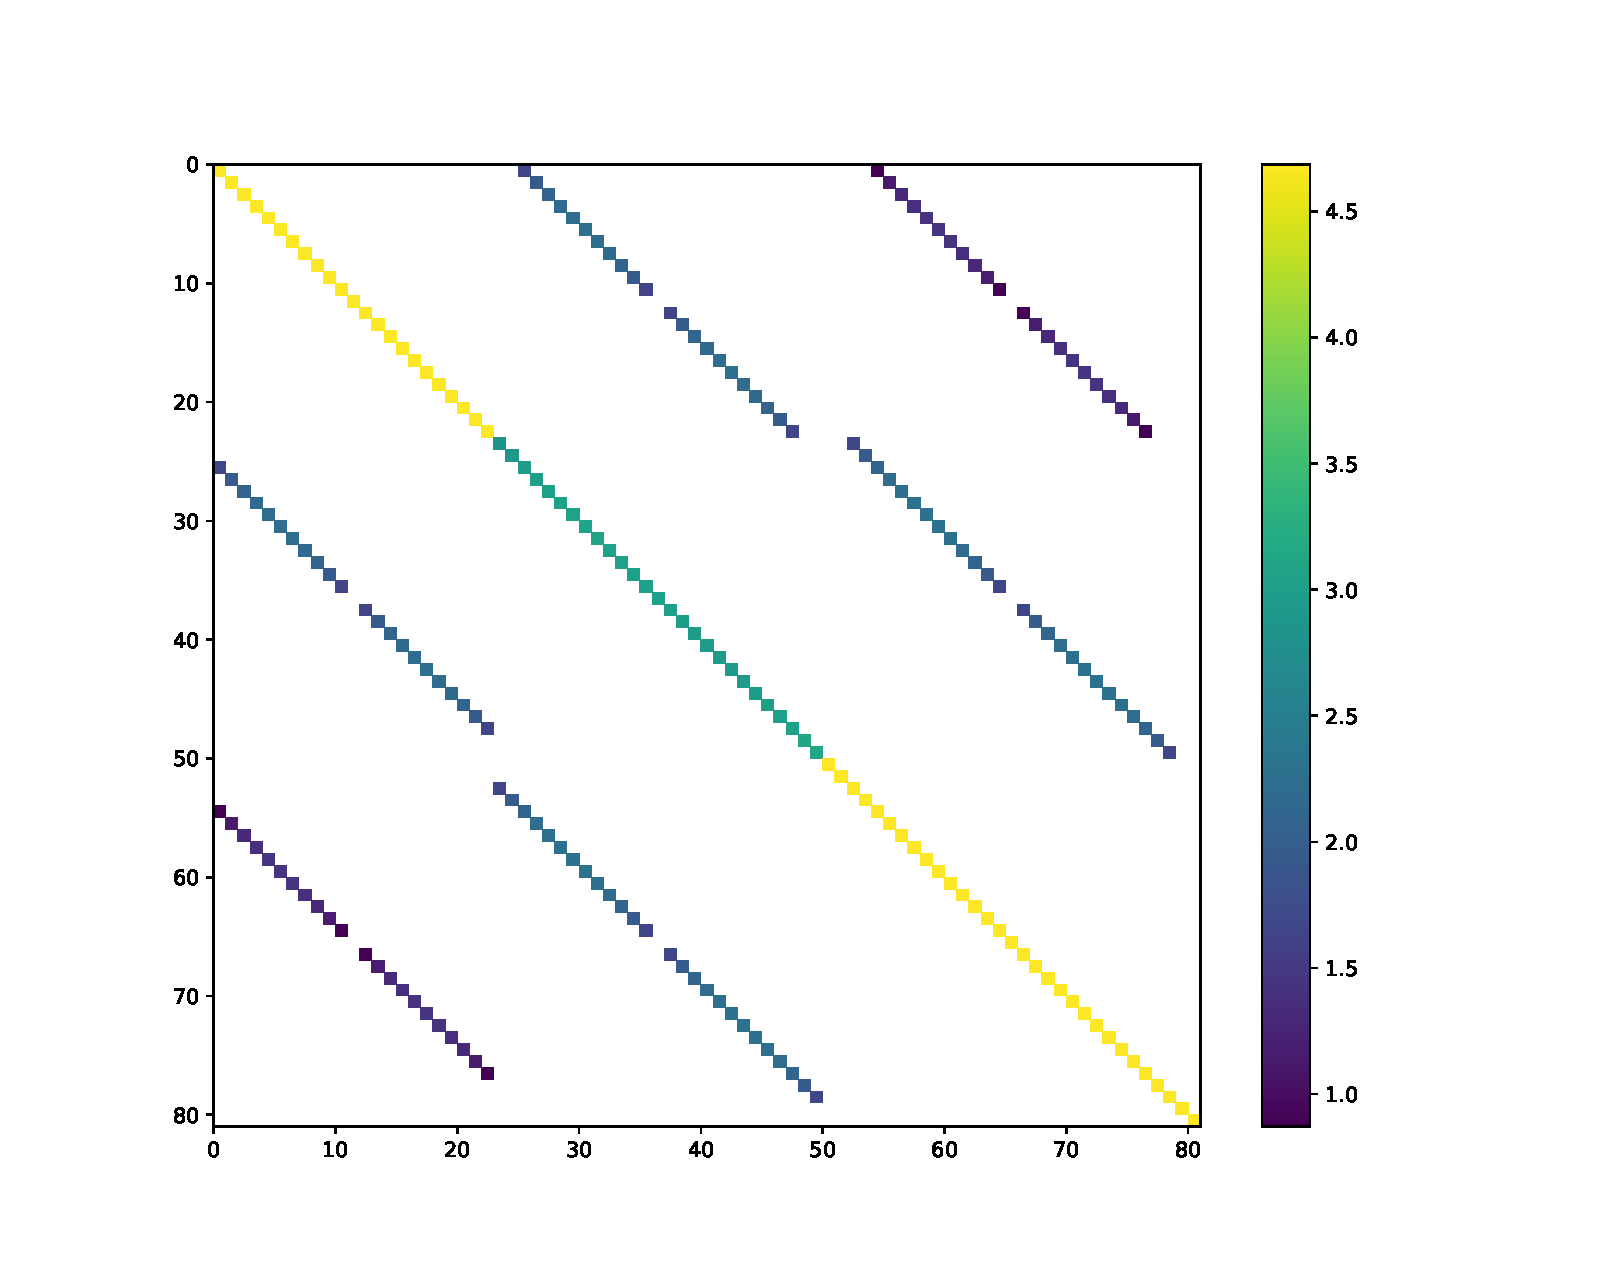
\includegraphics[scale=0.6,center]{Chapter2/figs/coup_mat}
\caption{Visualisation of $\log_{10}|Z_{k'k}|$ in $\mu Hz^2$ for the multiplets $\mode{0}{11}$, $\mode{0}{13}$, and $\mode{0}{15}$ with frequencies $603.69 \mu Hz$, $641.84\mu Hz$, and $677.55 \mu Hz$ respectively. Numbers on the X and Y axes represent cumulative $m$ of all three multiplets. White spaces correspond to $0$ value.}  
\label{fig:coup_mat}
\end{figure}
%!TEX root = ../thesis.tex
%*******************************************************************************
%****************************** Third Chapter **********************************
%*******************************************************************************
\chapter{Internal Magnetic Fields}

\section{Solar Magnetic Field}\label{mag_intro}

It is well known through the observation of much surface solar phenomenon like active regions, solar flares, coronal mass ejections etc, that the sun has in its interior, often highly localised, significant magnetic fields. The source of this magnetic field is theorised to be a primordial current which started a dynamo process that is kept going at the expense of continuous dissipation of energy from the solar bulk. It is also widely believed however that mean magnetic field throughout the solar bulk is fairly weak. This chapter is devoted to finding a method to observe signature of this magnetic field in the p-mode frequency spectrum.

Most of high intensity magnetic activity is limited to the solar surface. The tachocline is believed to contain toroidal fields as high as $10^5 \text{G}$. outside the tachocline the magnetic field is believed to be mostly dipolar such that mean surface magnetic field is about $10\text{G}$. Very strong time varying local magnetic fields apart from these are also known to exist near the surface, but detection of such time dependent fields is outside the scope of this work; here we shall only investigate the effects of steady fields.

%cite for tachocline B field
%cite for fairly weak B field
%cite for core B field
%cite for dynamo
\section{Equation of Motion}

In the presence of background magnetic field $\Bv$, the equation of motion is governed by the new operator $\cL \rightarrow \cL + \dL^{B}$, where $\dL^B$ is estabished in \cite{hanasoge17} as below.
\begin{align}
    \dLB \boldsymbol{\xi} &= \frac{-1}{4\pi}\boldsymbol{\nabla \cdot} [\Bv\Bv\cdot \boldsymbol{\nabla} \boldsymbol{\xi} + \Bv {\cdot} \boldsymbol{\nabla}\boldsymbol{\xi}\Bv - 2 \Bv\Bv\boldsymbol{\nabla \cdot}\boldsymbol{\xi} - (\boldsymbol{\xi \cdot \nabla} \Bv)\Bv - \Bv(\boldsymbol{\xi \cdot \nabla}\Bv)\notag
    \\& + B^2 \boldsymbol{\nabla \cdot \xi I} - \Bv\Bv :\boldsymbol{\nabla \xi I} + \boldsymbol{\xi \cdot \nabla}\frac{B^2}{2}\boldsymbol{I}] 
     \label{eqn:dLB}
\end{align}
where the $:$ stands for contraction of two second rank tensors ($\mathbf{P}:\mathbf{Q} \equiv P_{ij}Q_{ji} $).

Note that in above expression $\Bv$ only appears in the second order. \cite{goedbloed2004} contains a detailed derivation of this and a proof of self adjointedness for $\dL^B$.

This expression can be put in a more convenient form involving the Lorentz stress tensor $\cH \equiv \Bv\Bv$ as
\begin{equation} \label{eqn: mag_pert_H}
    \dLB \boldsymbol{\xi} = \frac{-1}{4\pi}\boldsymbol{\nabla\cdot} [\boldsymbol{\mathcal{H}\cdot\nabla \xi} + (\boldsymbol{\nabla \xi})^T \boldsymbol{\cdot \mathcal{H}} - 2\boldsymbol{\mathcal{H}\nabla \cdot \xi} - \boldsymbol{\xi \cdot \nabla \mathcal{H}} + \boldsymbol{\mathcal{H}:I \nabla \cdot \xi I} - \cH{:}\boldsymbol{\nabla \xi I} + \boldsymbol{\xi \cdot \nabla} \enc{\frac{\cH{:}\boldsymbol{I}}{2}}\boldsymbol{I}]
\end{equation}

\section{Coupling Matrix}
\subsection{Lorentz Stress components}\label{sec:lorentz_stress_comps}
The process of taking integrals over a sphere becomes simplified if we're operating in the Generalised Spherical Harmonics formalism. In this formalism (Appendix \ref{app_gsh}), magnetic field and Lorentz stress are decomposed as
$$\Bv = \sum_{st}\sum_{\alpha} B^{\alpha}_{st}(r) Y_{st}^{\alpha}(\theta,\phi) \ev{\alpha}$$
$$\cH = \sum_{st}\sum_{\mu\nu} h_{st}^{\mu\nu}(r) Y^{\mu+\nu}_{st}(\theta,\phi) \ev{\mu}\ev{\nu}$$
where the generalised spherical harmonic (GSH) coordinate indices given by Greek symbols run from $-1$ to $+1$.
Equation (\ref{eqn:h_B_relation}) relates the components of $\cH$ to $\Bv$. $\cH$ by construction satisfies the symmetry property $h^{\mu\nu}_{st} = h^{\nu\mu}_{st}$ ($\because \cH = \Bv\Bv$), and $\enc{h^{\mu\nu}_{st}}^* = (-1)^t h_{s\bar{t}}^{\bar{\mu}\bar{\nu}}$, where overbars represent negatives, follows from its realness condition.

\subsection{Sensitivity Kernels}\label{sec:mag_kern}
Coupling matrix element is given as on integral transform over $\cH$ as
\begin{equation}\label{lor_kernel_intro}
\LamB_{k'k} = \inner{\xiv_{k'}}{\dLB\xiv_{k}}=\int_0^{R_{\odot}} dr r^2 \sum_{\substack{st \\ \mu\nu}} \cB_{st}^{\mu\nu}(r) h_{st}^{\mu\nu}(r)
\end{equation}
where $\cB_{st}^{\mu\nu}$ are the eigenfunction dependent magnetic sensitivity kernels. Prescription for evaluating these kernels and the explicit expressions can be found in \cite{hanasoge17}. It should be noted however that the coupling integral $\inner{\xiv_{k'}}{\dLB\xiv_{k}}$ can be reduced to the radial integral form obtained in  (\ref{lor_kernel_intro}) contains no boundary terms. It is indeed the case that the magnetic field is assumed to vanish at the surface in this analysis. Relaxing this assumption will introduce boundary terms which involve integrals only over the solar surface.
Since $h_{st}^{\mu\nu}$ is symmetric in interchange of $\mu$ and $\nu$, we may ascribe the same symmetry to $\cB_{st}^{\mu\nu}$ too without any loss in generality.

Using the Mathematica package developed for this work \cite{GSH_repo} which automates manipulation of tensor spherical harmonics via the method of GSHs, the following forms of the kernels were found

\begin{dmath}\label{eq:kern_mm}
\cB_{st}^{--} = \frac{(-1)^{m'+1}}{r^2}\gam{l}\gam{l'}\gam{s}\wigred{-m'}{t}{m} \enccrl{\wigred{1}{-2}{1}\om{l}{0}\om{l'}{0} \encsqr{\enc{U+{\om{l'}{2}}^2 V}V' - UU'-rV\dot{V}'} +\wigred{2}{-2}{0} \om{l'}{0}\om{l'}{2}\encsqr{(U+r\dot{U})V'-rU\dot{V}'} +\wigred{0}{-2}{2} \om{l}{0}\om{l}{2}rV\dot{U}' + \wigred{3}{-2}{-1} \om{l}{0}\om{l'}{0}\om{l'}{2}\om{l'}{3}VV'}   
\end{dmath}

\begin{dmath}\label{eq:kern_0m}
2\cB_{st}^{0-} = \frac{(-1)^{m'}}{r^2}\gam{l}\gam{l'}\gam{s}\wigred{-m'}{t}{m} \enccrl{\wigred{0}{-1}{1}\om{l}{0}\encsqr{\enc{2U+{\om{l'}{2}}^2 V}U' +{\om{l'}{0}}^2 \enc{-2UV'-VV'+rV\dot{V}'} -r\enc{U+V-r\dot{V}'}\dot{U}'} - \wigred{1}{-1}{0}\om{l'}{0}\encsqr{(-2U+{\om{l}{0}}^2V)U' + {\om{l}{0}}^2V\enc{r\dot{V}'-V'} + U\enc{2V' + r (\dot{U}' - 2\dot{V}' + r\ddot{V}')}}  +\wigred{-1}{-1}{2}\om{l}{0}\om{l'}{0}\om{l}{2}V\encsqr{U'-V'+r\dot{V}'} + \wigred{2}{-1}{-1}\om{l}{0} \om{l'}{0} \om{l'}{2}\encsqr{V\enc{U'-3V'+r\dot{V}'}+2r\dot{V}V'}}  
\end{dmath}

\begin{dmath}\label{eq:kern_00}
\cB_{st}^{00} = \frac{(-1)^{m'}}{2r^2}\gam{l}\gam{l'}\gam{s}\wigred{-m'}{t}{m} \enc{1+p}\enccrl{\frac{1}{2}\wigred{0}{0}{0}\encsqr{ \enc{6U-4{\om{l}{0}}^2 V-2 r \dot{U}} \enc{U'-{\om{l'}{0}}^2V'} + 2{\om{l'}{0}}^2 rU\dot{V}' + r\enc{\enc{-4U+2{\om{l}{0}}^2V+r\dot{U}}}\dot{U}'+rU\ddot{U}' } -\wigred{-1}{0}{1}\om{l'}{0}\om{l}{0} \encsqr{V\enc{-4U'+2\enc{1+{\om{l'}{0}}^2} V'+r\enc{\dot{U}'-2\dot{V}'}} +2r\dot{V}\enc{U'-V'+r\dot{V}'}}
} 
\end{dmath}

\begin{dmath}\label{eq:kern_pm}
2\cB_{st}^{+-} = \frac{(-1)^{m'}}{r^2}\gam{l}\gam{l'}\gam{s}\wigred{-m'}{t}{m}\enc{1+p} \enccrl{-2\wigred{-2}{0}{2}\om{l}{0}\om{l}{2} \om{l'}{0}\om{l'}{2} VV' + \wigred{-1}{0}{1}\om{l'}{0}\om{l}{0}\encsqr{-rV\dot{U}' + U \enc{U'-V'+r\dot{V}'}} 
+\wigred{0}{0}{0}r^2\encsqr{U\ddot{U}'-\dot{U}\dot{U}'}
}  
\end{dmath}
where $p \equiv (-1)^{l'+l+s}$, $U,V \equiv U_{nl},V_{nl}$, and $U',V' \equiv U_{n'l'},V_{n'l'}$.
\clearpage
Kernel components $\cB_{st}^{\mu\nu}$ are found to have these following properties:
\begin{enumerate}
\item $\cB_{st}^{\mu\nu} = \cB_{st}^{\nu\mu}$ (by construction)
\item $\cB_{st}^{--} = (-1)^{l+l'+s}\cB_{st}^{++}$
\item $\cB_{st}^{0-} = (-1)^{l+l'+s}\cB_{st}^{+0}$
\item $\cB_{st}^{00} = \cB_{st}^{+-}=\cB_{st}^{-+}=0$ for odd $\enc{l'+l+s}$
\end{enumerate}

\begin{figure}[t]
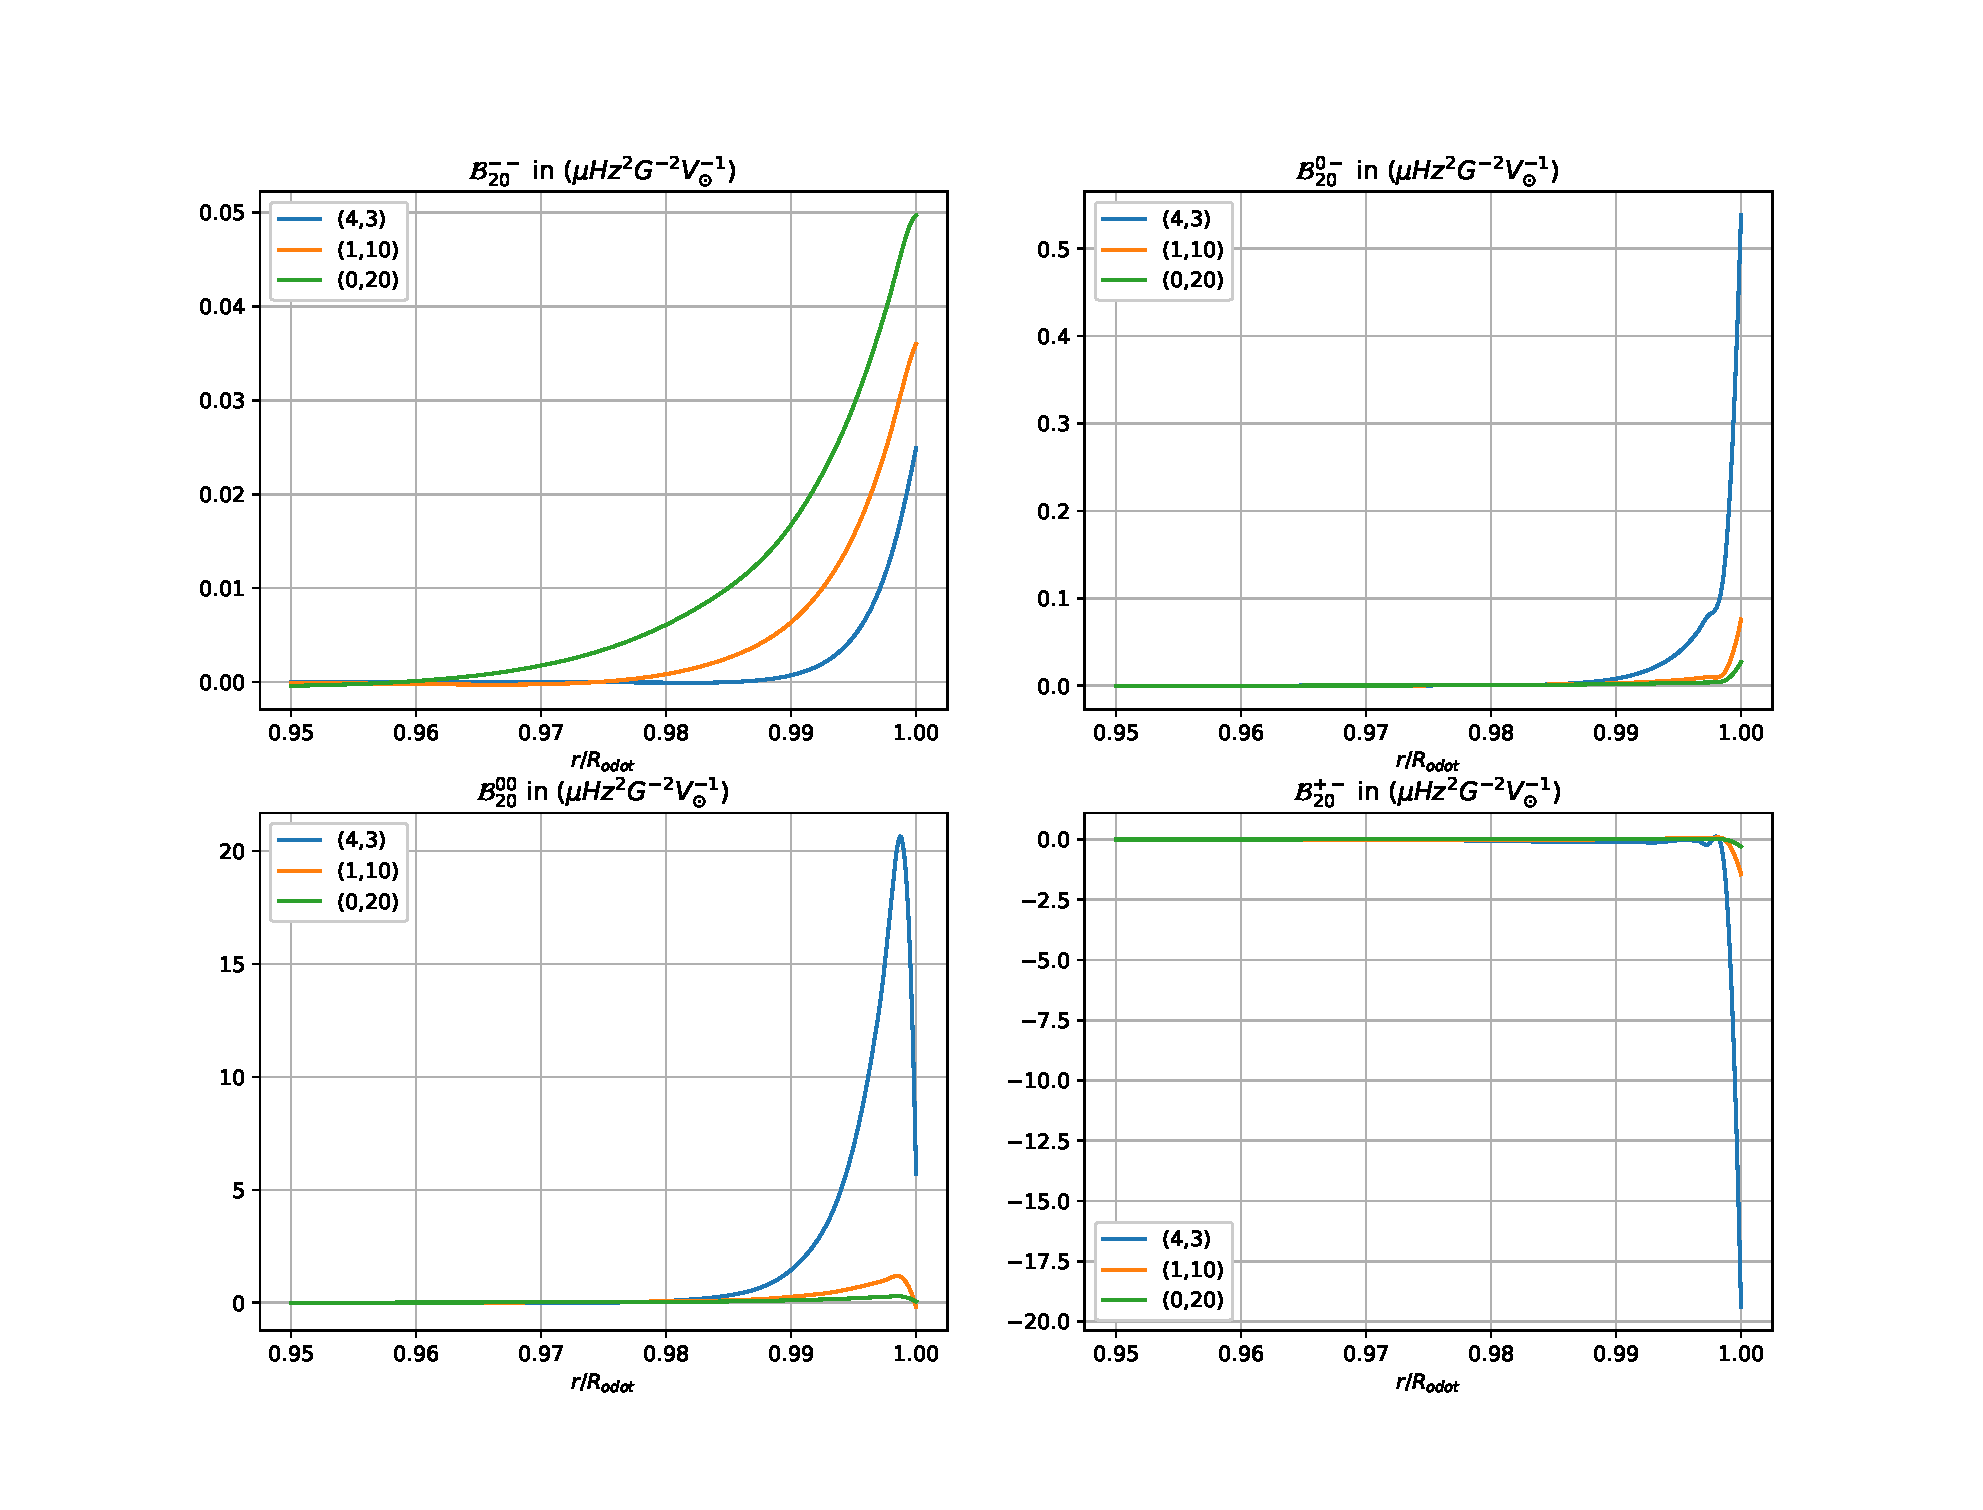
\includegraphics[scale=0.55,center]{Chapter3/figs/kern_self.eps}
\caption{Self coupling Kernels for the modes $\mode{4}{3}$, $\mode{1}{10}$, and $\mode{0}{20}$.}
\label{fig:kern_plot}
\end{figure}

Figure (\ref{fig:kern_plot}) shows the four independent components of the sensitivity kernel under self coupling for some modes. It is clear from the plots that for all modes, sensitivity is mostly localised to the solar boundary. This effect is most striking for $\cB^{+-}_{st}$ across modes. This is a an indirect consequence of the background density profile of the sun which falls almost exponentially fast with respect to radius towards the outer regions of the sun. The low density near the boundary makes the eigenfunction peak distinctly near the boundary. However, as can be seen in equations (\ref{eq:kern_mm}) - (\ref{eq:kern_pm}), the kernels depend quadratically on $U$ and $V$, which finally makes them peak at the boundary. This implies that most of the magnetic splitting caused is due to the fields near the surface and acts as limitation to imaging the interior magnetic field precisely via an inversion of frequency splitting data.

We can see that how it is ultimately the components of $\cH$ that couple with the sensitivity kernel; components of $\Bv$ cannot be related to frequency splittings in a straightforward manner like equation (\ref{lor_kernel_intro}). Hence, any procedure inverting splitting data will first determine the $\cH$ components. It remains unclear if the magnetic field can be recovered from just the knowledge of components of $\cH$.

\section{Synthetic Magnetic Field}
Using some basic pieces of information about mean solar magnetic field as given in \ref{mag_intro}, we can posit the following form of a synthetic magnetic field which will be used for validating our routine of finding frequency splits. We give the following form of the magnetic field which is comoposed of an internal toroidal field concentrated at the core and the tachocline, and a dipolar field which extends from the tachocline to the surface.

\subsection{Construction of $\Bv$}\label{sec:B_construction}
Using the identities $\grad_1 Y_l^m = \om{l}{0} \enc{Y_{lm}^{-1} \ev{-} + Y_{lm}^{1} \ev{+}}$, $\ev{r} \times\grad_1 Y_l^m = i\om{l}{0} \enc{Y_{lm}^{-1} \ev{-} - Y_{lm}^{1} \ev{+}}$, and $Y_1^0(\theta,\phi) = \gam{1}\cos\theta$ we see following things: (1) A toroidal field $\Bv = \alpha(r) \sin\theta \ev{\phi}$ can be given as $B_{10} = i \alpha(r) / \gam{1} \enc{-1,0,1}$ with all other $B_{st}$ components being $0$, and (2) A dipolar field $\Bv = \beta(r) (2\cos\theta \ev{r} + \sin\theta\ev{\theta})$ with $\beta \propto r^{-3}$ can be given as $B_{10} = -\beta(r)/\gam{1} \enc{1,-2,1}$ with all other $B_{st}$ components being $0$. Note that the row vector refers to the GSH coordinate index $\mu$. This leads to the following final form of $\Bv$

\begin{equation}\label{mag_field}
B_{st}(r) = 
\begin{cases}
-i \frac{\alpha(r)}{\gam{1}} \gshvec{1}{0}{-1}  - \frac{\beta(r)}{\gam{1}} \gshvec{b-r\dot{b}}{-2b}{b-r\dot{b}}, & \text{for} (s,t) = (1,0) \\
0, & \text{for} (s,t) \neq (1,0)
\end{cases}
\end{equation}
where $b(r)=1$ where field is perfectly dipolar. The term $r\dot{b}(r)$ appear as a consequence of fixing the diveregence to zero and is only nonzero in the transition region where $b(r)$ goes from $0$ to $1$. It was can be checked via using $\grad \cdot \Bv = g_{\alpha\beta} (\grad\Bv)^{\alpha\beta}$ (\cite{GSH_repo} was used) that the two parts in (\ref{mag_field}) (toroidal and dipolar) satisfy the solenoidal condition independently. We plot the forms of the $\alpha$, $\beta$, and $b$ used in our frequency splitting calculations.

\begin{figure}[t]
\begin{subfigure}{0.5\linewidth}
\centering
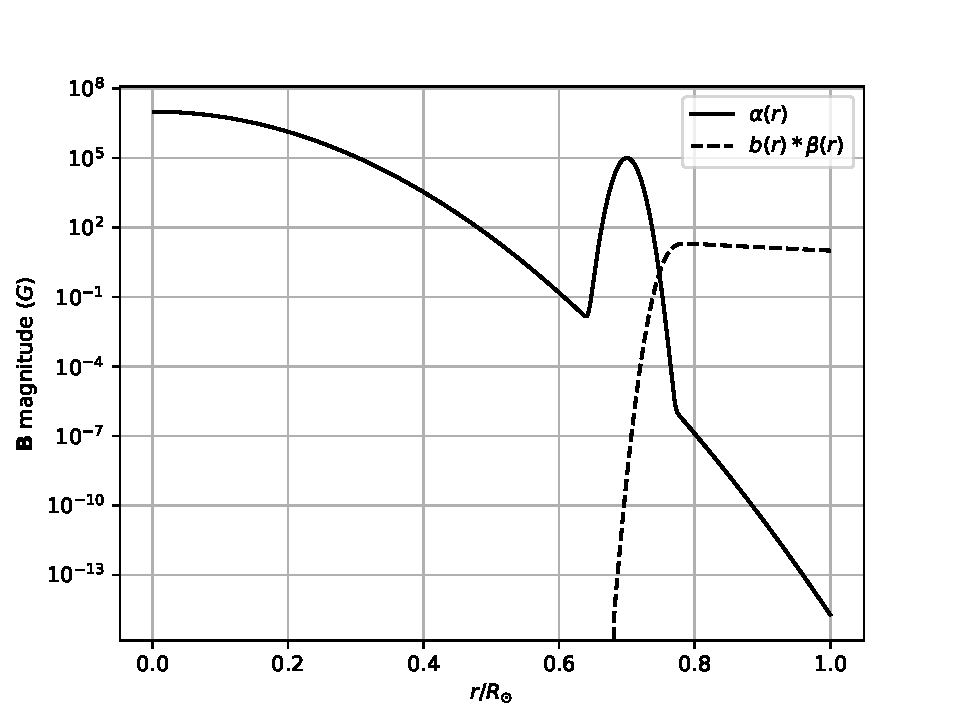
\includegraphics[scale=.5]{Chapter3/figs/alpha_beta}
\caption{$\alpha(r)$ and $b(r) \beta(r)$ in $G$}
\label{fig:alpha_beta}
\end{subfigure}
\begin{subfigure}{0.5\linewidth}
\centering
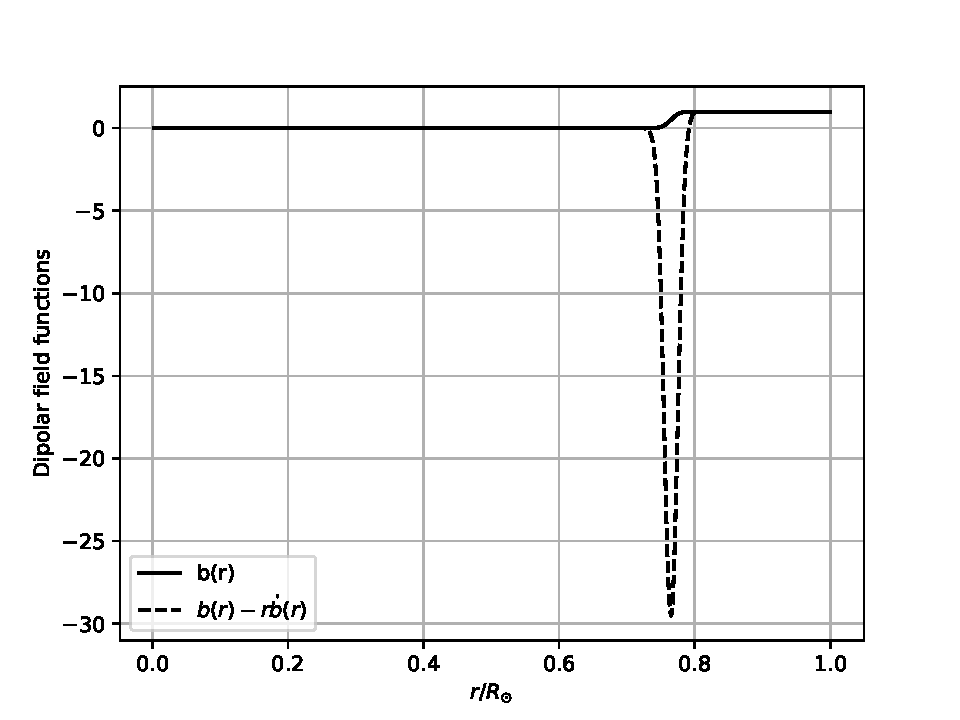
\includegraphics[scale=0.5,center]{Chapter3/figs/b}
\caption{$b(r)$ and $a(r) = b(r)-r\dot{b}(r)$}
\label{fig:a_b}
\end{subfigure}
\caption{$\alpha(r)$ is addition of two Gaussians centred at $r=0$ with peak $10^7 G$ and at $r=0.7R_{\odot}$ with peak $10^5 G$ respectively. $b$ transitions smoothly from $0$ to $1$ as a sigmoid around $r=0.7R_{\odot}$. $r=0.7R_{\odot}$ mark is roughly where the tachocline is placed. Figure (\ref{fig:alpha_beta}) shows the poloidal (dipolar) field $\beta$ starting to dominate over the toroidal field by atleast three orders of magnitude as $r$ exceeds $\sim 0.8 R_{\odot}$.}
\end{figure}

\subsection{Construction of $\mathcal{H}$}

After the form of $\Bv$ has been ascertained, it is straighforward to derive components of $\cH$ via taking a tensor product. Decomposing either field in their GSH forms as in \ref{sec:lorentz_stress_comps}, and using orthonormality relation
\begin{equation}
\int d\Omega \enc{Y_{l_1m_1}^{n_1}}^*Y_{l_2m_2}^{n_2} = \delta_{l_1l_2}\delta_{m_1m_2}\delta_{N_1N_2}
\end{equation}

and the triple integral result

\begin{equation}\label{eq:triple_integral}
\int d\Omega \enc{Y_{l_1m_1}^{N_1}}^*Y_{l_2m_2}^{N_2}  Y_{l_3m_3}^{N_3}= (-1)^{m_1+N_1}4\pi \gam{l_1}\gam{l_2}\gam{l_3} \wigfull{l_1}{l_2}{l_3}{-m_1}{m_2}{m_3} \wigfull{l_1}{l_2}{l_3}{-N_1}{N_2}{N_3}
\end{equation}

one can write
\begin{equation}
h^{\mu\nu}_{st} = \sum_{\substack{s_1t_1\\ s_2t_2}} \langle Y_{st}^{\mu+\nu}, Y_{s_1 t_1}^{\mu}  Y_{s_2 t_2}^{\nu}\rangle B_{s_1t_1}^{\mu} B_{s_2t_2}^{\nu}
\label{eqn:h_B_relation}
\end{equation}
Where $\langle Y_{l_1m_1}^{n_1}, Y_{l_2m_2}^{N_2}  Y_{l_3m_3}^{N_3}\rangle$ stands for the integral in equation (\ref{eq:triple_integral}).
If $\Bv$ has only $s=s_0$ and $t=t_0$ features, that is $\Bv = \sum_{\alpha}B_{s_0t_0}^{\alpha}Y_{s_0t_0}^{\alpha} \ev{\alpha}$, components of $\cH$ are given by
\begin{equation}\label{eq:single_feature_B}
h_{st}^{\mu\nu} = B^{\mu}_{s_0 t_0}B^{\nu}_{s_0 t_0} (-1)^{\mu + \nu + t} (2s_0+1) \gam{s} \wigfull{s_0}{s}{s_0}{\mu}{-(\mu+\nu)}{\nu} \wigfull{s_0}{s}{s_0}{t_0}{-t}{t_0}
\end{equation}

For the axis symmetric magnetic field constructed in \ref{sec:B_construction}, we may set $s_0=1$ and $t_0=0$. Wigner 3j selection rules given in \ref{sec:selec_rules} dicate that $\cH$ can only have $s=0,1,2$ and $t=0$. Then we have the form
 	
\begin{equation}
h_{s0}^{\mu\nu} = 3 \gam{s} B^{\mu}_{10}B^{\nu}_{10} (-1)^{\mu + \nu} \wigfull{1}{s}{1}{\mu}{-(\mu+\nu)}{\nu} \wigfull{1}{s}{1}{0}{0}{0}
\end{equation}

But we know that $\wigfull{1}{s}{1}{0}{0}{0}$ vanishes for odd s. Thus we note here that $\cH$ has no $s=1$ and has non-zero $s=0$ components, which is different from how differential rotation couples modes. The $s=0$ feature of the Lorentz stress tensor indicates a net shift from the unperturbed mode frequency $\omega_{{nl}}$ for a particular multiplet $\mode{n}{l}$ as this term couples with $\wigfull{l'}{0}{l}{-m}{0}{m}$ which is independent of $m$.
\chapter{Results}  %Title of the First Chapter

\ifpdf
    \graphicspath{{Chapter1/Figs/Raster/}{Chapter1/Figs/PDF/}{Chapter1/Figs/}}
\else
    \graphicspath{{Chapter1/Figs/Vector/}{Chapter1/Figs/}}
\fi

\section{Frequency Splittings due to Differential Rotation} %Section - 1.1 
In this treatment we show that while taking very closely spaced multiplets, the isolated multiplet condition breaks down and there is significant cross coupling across modes due to differential rotation alone. Because axis symmetry imposes the $m'=m$ selection rule, the supermatrix $Z_{k'k}$ of perturbation $\dLd$ is a sparse matrix consisting of diagonals and subdiagonal as show in figure (\ref{fig:coup_mat}). As a case study, we choose to investigate the splitting coefficients of the mode $\mode{0}{77}$ as a result of cross coupling with its neighbouring modes which all lie withing an interval of $100\mu Hz$.

\subsection{Splitting with pure rotation}
We plot the split frequencies $\mode{0}{77}$ along with some neighbouring modes to contrast the results obtained from a QDPT and a DPT analysis.

\begin{table}
\begin{center}
\begin{tabular}{|l|c|c|c|c|c|c|c|c|r|}
\hline
$_n\bm{S}_l$ 
& \mode{0}{69}
& \mode{0}{71}  
& \mode{0}{73} 
& \mode{0}{75} 
& \mode{0}{77} 
& \mode{0}{79} 
& \mode{0}{81}  
& \mode{0}{83} 
& \mode{0}{85}
\\ \hline
$\bm{\omega}_{nl}$ 
& \hfill 848.219 
& \hfill 860.008 
& \hfill 871.636 
& \hfill 883.110 
& \hfill 894.434 
& \hfill 905.615 
& \hfill 916.659 
& \hfill 927.570 
& \hfill 938.353  \\ 
\hline

\end{tabular}
\end{center}
\caption{Frequencies in $\mu Hz$ corresponding to all modes discussed in this chapter. These modes have been chosen to be in increasing order in frequency and satisfying the $\delta l  =2$ condition.}
\label{tab:mode_list}
\end{table}

\begin{figure}[h!]
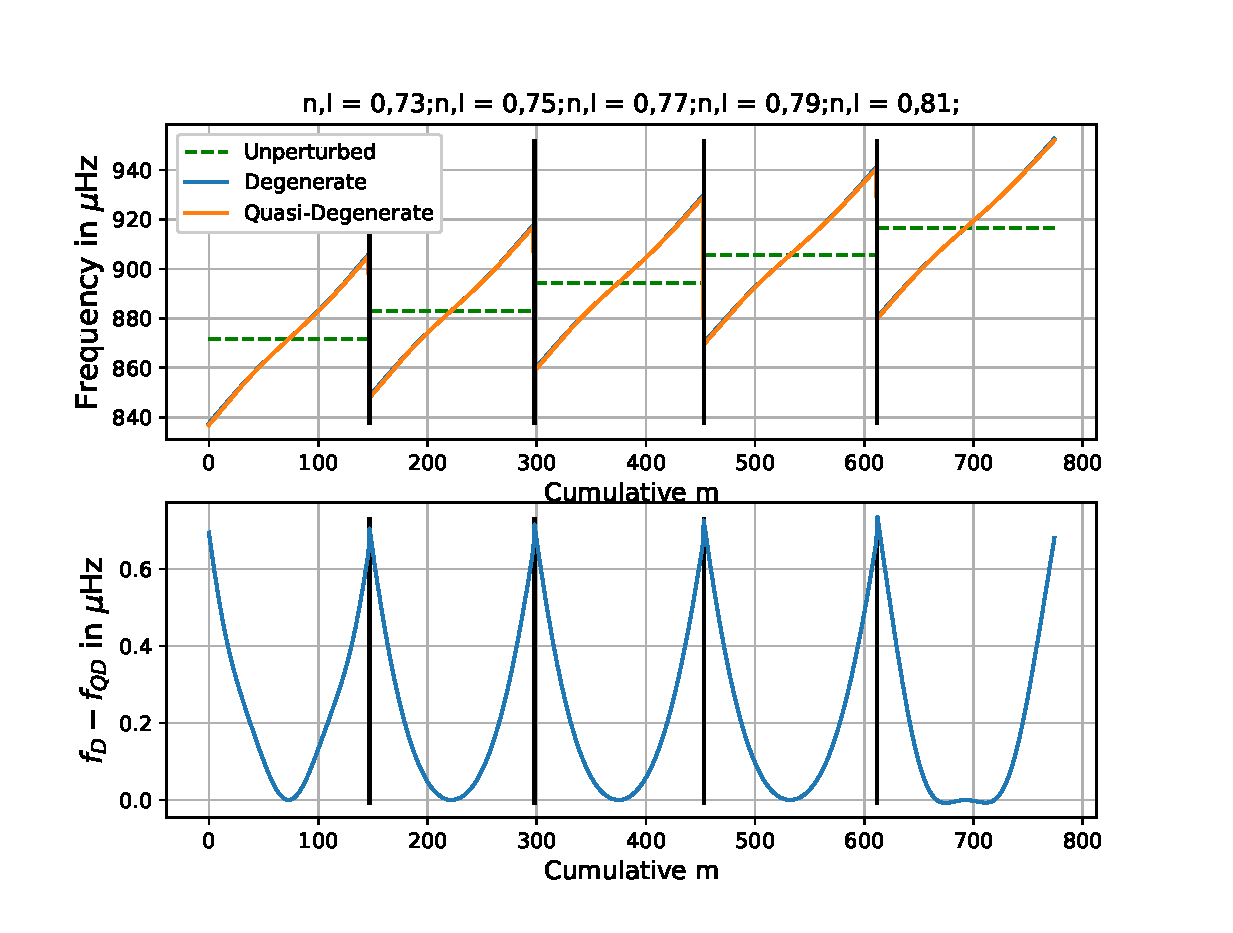
\includegraphics[scale=0.8,center]{Chapter4/figs/dr_split}
\caption{DPT and QDPT splits with $\mode{0}{73}$, $\mode{0}{75}$, $\mode{0}{77}$, $\mode{0}{79}$, and $\mode{0}{81}$ which have frequencies 871.63$\mu Hz$, 883.12$\mu Hz$, 894.43$\mu Hz$, 905.62$\mu Hz$, and 916.66$\mu Hz$ respectively. Top plot shows frequency splittings of the five modes and their unperturbed frequencies (green dashed). DPT and QDPT lie indiscernably   Bottom plot shows the departure of the DPT frequencies from the dpt frequencies.}
\label{fig:split_dr}
\end{figure}

$a$-coefficients obtained from the split is tabulated in table \ref{tab:split_dr}. $a_1$'s found from QDPT and DPT come out to be close to $440nHz$ which is corresponds to the $24$ day rotational cycle of the sun. $a_3$ and $a_5$ are found to be in good agreement upto a tolerance of $1nHz$. However, the QDPT profile contains even $a$-coefficients of the order of $5nHz$. This leads to an even profile departure of the QDPT from DPT profile of the order of $600nHz$ in the frequency spectrum as shown in figure (\ref{fig:split_dr}).

\begin{table}
\begin{center}
\begin{tabular}{|l|c|r|}
\hline
\textbf{Mode} & \textbf{QDPT(nHz)} & \textbf{DPT(nHz)} \\ \hline
$a_0$ &\hfill -2.832 & \hfill  - \\ \hline
$a_1$ & \hfill 438.378 & \hfill 438.178 \\ \hline
$a_2$ & \hfill -5.876 & \hfill - \\ \hline
$a_3$ & \hfill 22.149 & \hfill 22.005 \\ \hline
$a_4$ & \hfill -0.308 & \hfill  - \\ \hline
$a_5$ & \hfill -4.925 & \hfill -4.934 \\ \hline
$a_6$ & \hfill 0.091 & \hfill - \\ \hline
$a_7$ & \hfill -0.002 & \hfill  - \\ \hline
$a_8$ & \hfill -0.018 & \hfill - \\ \hline
$a_9$ & \hfill - & \hfill  - \\ \hline
$a_{10}$& \hfill  0.004 & \hfill  - \\ \hline
\end{tabular}
\end{center}
\caption{Splitting coefficients for mode $\mode{0}{77}$ via QDPT and DPT analysis. Hyphens stand for values $< 0.001nHz$.}
\label{tab:split_dr}
\end{table}

\subsection{Splitting with pure rotation removed}
We see that the component $w_1^0(r)$ in the sun's rotational profile gives rise to a velocity field
$$\mathbf{v} = -w_1^0 \partial_{\theta}Y_1^0 \ev{\phi} = \gam{1}w_1^0 \sin\theta \ev{\phi}$$
which corresponds to pure shell like rotation at each particular radius $r$. Taking $w_1^0 \rightarrow w_1^0 - \Omega_1 r / \gam{1}$ gives
\begin{equation}
\mathbf{v} = \gam{1}w_1^0 \sin\theta \ev{\phi} - \Omega_1 r \sin\theta \ev{\phi}
\end{equation}
and hence corresponds to slowing down each shell by an angular velocity $\Omega_1$ about the spin axis. Thus, subtracting out $\Omega_1 r / \gam{1}$ from $w_1^0$ is equivalent to slowing down the pure rotational profile by angular velocity $\Omega_1$.

We see that after removing an pure rotation component equivalent to 440nHz from the $w_1^0$ rotational profile, we get the following splitting of frequencies for QDPT and DPT respectively as shown in figure (\ref{fig:split_dr}). QDPT is performed taking 5 modes all lying in a band of width $100\mu Hz$.
\begin{figure}[h!]
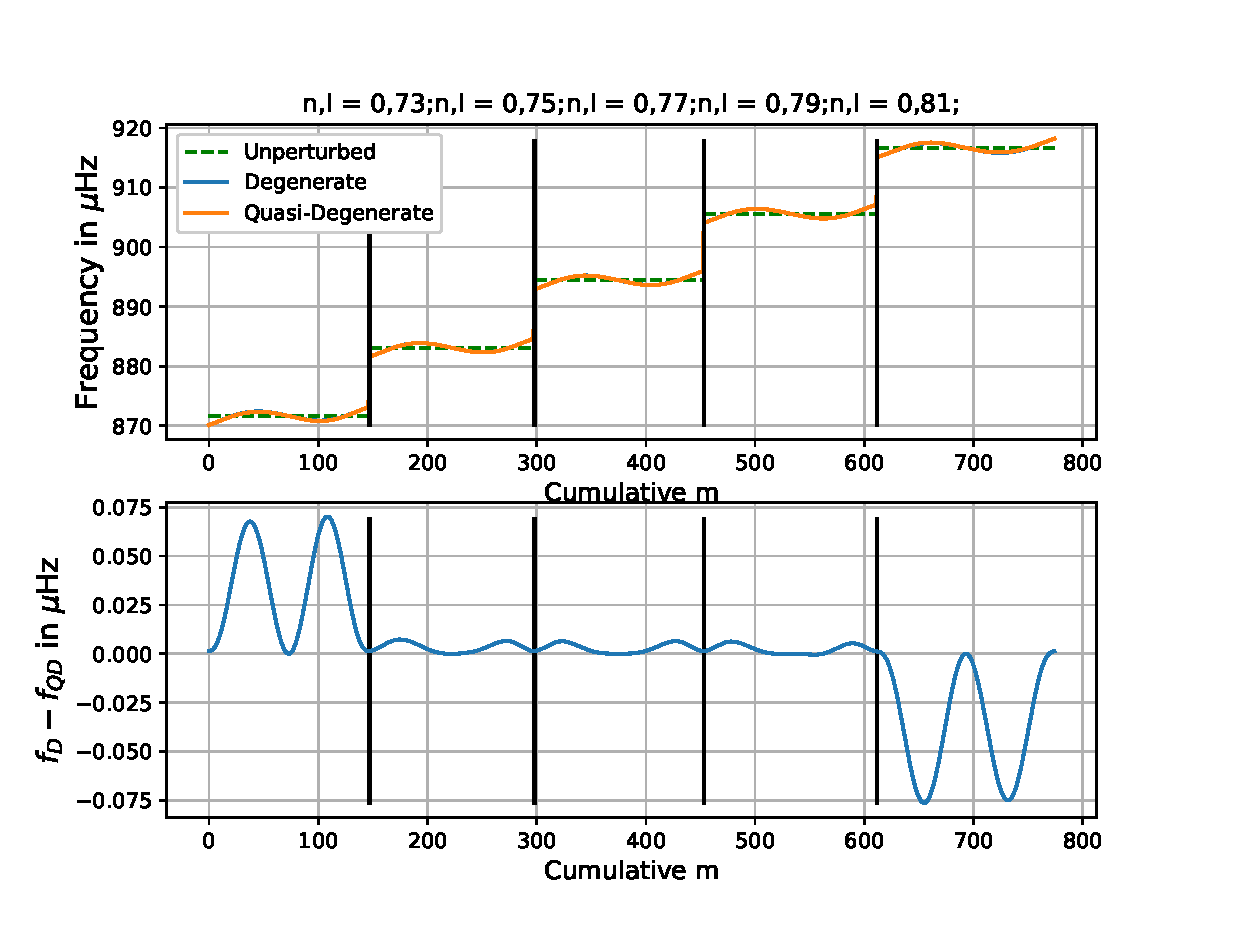
\includegraphics[scale=0.8,center]{Chapter4/figs/dr_split_rm}
\caption{DPT and QDPT rotational splits with pure rotational component equivalent to $440 nHz$ removed from $w_1^0$ for modes $\mode{0}{73}$, $\mode{0}{75}$, $\mode{0}{77}$, $\mode{0}{79}$, and $\mode{0}{81}$ which have frequencies as shown in table (\ref{tab:mode_list}). Top plot shows frequency splittings of the five modes and their unperturbed frequencies. Bottom plot shows the departure of the QDPT frequencies from the DPT frequencies.}
\label{fig:split_dr_rm}
\end{figure}

\begin{table}
\begin{center}
\begin{tabular}{|l|c|r|}
\hline
\textbf{Mode} & \textbf{QDPT(nHz)} & \textbf{DPT(nHz)} \\ \hline
$a_{0}$ & \hfill -0.038 &\hfill  - \\ \hline
$a_{1}$ & \hfill  2.820 &\hfill  2.820 \\ \hline
$a_{2}$ & \hfill -0.030 &\hfill - \\ \hline
$a_{3}$ & \hfill 22.005 &\hfill 22.005 \\ \hline
$a_{4}$ & \hfill  0.071 &\hfill  - \\ \hline
$a_{5}$ & \hfill -4.933 &\hfill -4.934 \\ \hline
$a_{6}$ & \hfill -0.006 &\hfill  - \\ \hline
$a_{7}$ & \hfill  - &\hfill  - \\ \hline
$a_{8}$ & \hfill -0.018 &\hfill - \\ \hline
$a_{9}$ & \hfill - &\hfill  - \\ \hline
$a_{10}$ & \hfill  0.004 &\hfill  - \\ \hline
\end{tabular}
\end{center}
\caption{Splitting coefficients for the splitting of mode $\mode{0}{77}$ by QDPT and DPT analysis after removing pure rotational component equivalent to $440nHz$ from $w_1^0$. Hyphens stand for values $< 0.001nHz$.}
\label{tab:split_dr_rm}
\end{table}

\subsubsection{QDPT vs DPT with increasing coupling modes}
When QDPT is performed taking multiple neighbouring modes amongst the ones in table \ref{tab:mode_list}, a peculiar trend is found when comparing QDPT frequencies with theri DPT counterparts for each singlet mode. The trend in figure (\ref{fig:DPT_err}) shows large deviations in QDPT splitting from from DPT frequencies in modes placed at either extreme regardless of how many modes couple while QDPT-DPT departure in the inner modes stay the same. This hints at the large QDPT-DPT frequency differences obtained for the extremal modes being artefacts of the calculation and hence being unreliable. For reference henceforth, we only use QDPT frequencies of $\mode{0}{77}$ which remains relatively unchanged with respect to number of modes being considered.

\begin{figure}[h]
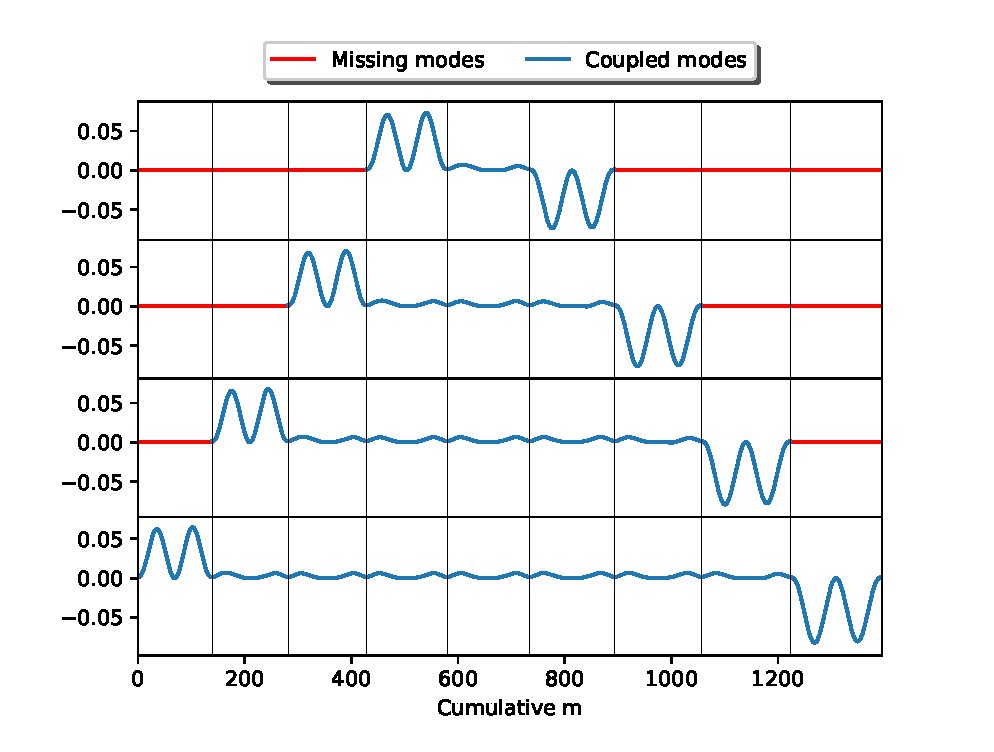
\includegraphics[scale=0.9, center]{Chapter4/figs/qdpt_err}
\caption{(QDPT - DPT) deviation with differing number of neighbouring modes being allowed to couple via differential rotation with mean rotation removed. From top, $\mode{0}{77}$ is made to couple with two, four, six, and eight closest $\Delta l=2$ neighbours (by frequency) as listed in table \ref{tab:mode_list}.}
\label{fig:DPT_err} 
\end{figure}

\section{Splittings due to Lorentz Stresses} %Section - 1.2

For finding magnetic splitting of the frequency spectrum, we choose to go to the corotating frame ($440 nHz$) to eliminate the dominant linear trend from the splitting profile and perform QDPT with the perturbation $\dLB$ on a background spectrum which is already split by differential rotation. We are justified in doing this because eliminating a net rotational component is equivalent to a coordinate transformation \cite{jcd_notes}. In this treatment where the background profile is already  split by differential rotation, our perturbation which couples different modes is $\dLB$ (equation  (\ref{eqn:dLB})). Background frequencies $\omega_{nlm}$ are obtained by performing DPT on degenerate modes $\mode{n}{l}$. We have chosen to perform DPT over QDPT for obtaining background $\omega_{nlm}$'s to reduce computational burden because resultant frequencies differ by less than $10nHz$ (centre section of figure (\ref{fig:split_dr_rm}) corresponding to $\mode{0}{77}$) and odd $a$-coefficients are almost identical (table \ref{tab:split_dr} shows the low relative error in odd $a$-coefficients).

The departure from the (rotating) background of the spectrum is shown in figure (\ref{fig:mag_split}). The $a$-coefficients are listed in table \ref{tab:mag_split}. The table also contains the $a$-coefficients for magnetic splitting obtained from QDPT performed on a background with no rotation for comparison.

\begin{figure}[h!]
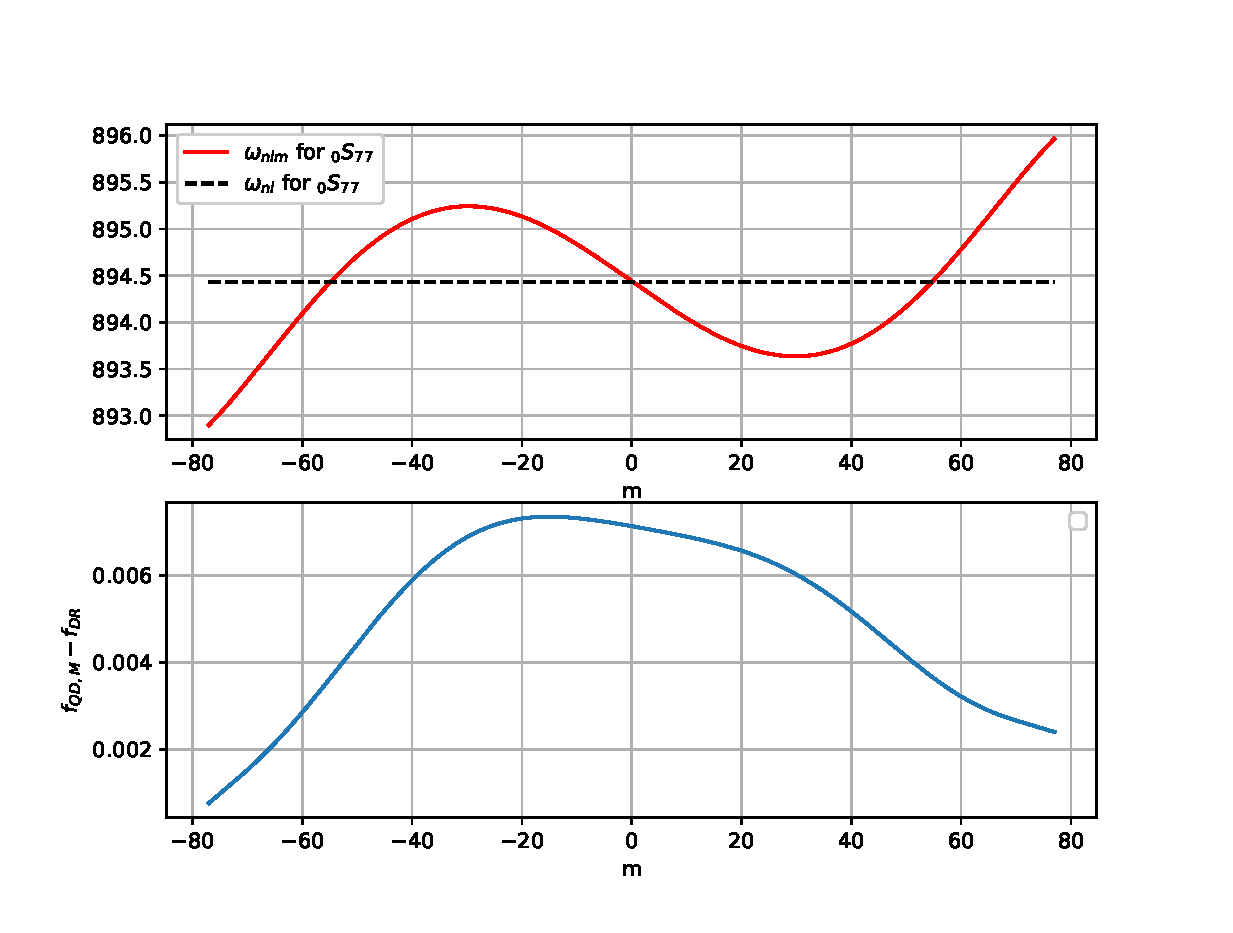
\includegraphics[scale=0.9, center]{Chapter4/figs/mag_split}
\caption{Magnetic splitting profile of the mode \mode{0}{77} obtained from QDPT containing all nine modes listed in table \ref{tab:mode_list} on rotating background with $440nHz$ equivalent component removed from $w_1^0$. Top shows the absolute frequency about the unperturbed baseline in $\mu HZ$. Bottom shows the difference between the overall (rotation + magnetic field) and the background rotation profile obtained from DPT.}
\label{fig:mag_split}
\end{figure}

\subsection{Detectibility}
the first two columns of table \ref{tab:mag_split} show the effect of magnetic perturbation on even $a$-coefficients. While the non-magnetic rotating profile (obatined by DPT) contains no evn $a$'s at all, the magnetic perturbation introduces $a_0=63 pHz$ and $a_2=-59pHz$. These $pHz$ level $a$-coefficients are not detectable by current standards of precision in observation as minimum errors in observed coefficients lie in the $\sim 1nHz$ range \cite{schou_data}.

\begin{table}
\begin{center}
\begin{tabular}{|l|c|c|r|}
\hline
\textbf{$\bm{a}_n$} & \shortstack{\textbf{Magnetic QDPT} \\ \textbf{(on rotating} \\ \textbf{ background)}} & \shortstack{\textbf{Rotating} \\ \textbf{ Background} \\ \textbf{(no magnetic field)}} & \shortstack{\textbf{Magnetic DPT} \\ \textbf{(on stationary} \\ \textbf{ background)}} \\ \hline
$a_{0}$ & \hfill  0.063 & \hfill - & \hfill  0.061 \\ \hline
$a_{1}$ & \hfill  2.822 & \hfill  2.820 &\hfill  - \\ \hline
$a_{2}$ & \hfill -0.059 & \hfill - & \hfill -0.059 \\ \hline
$a_{3}$ & \hfill 22.020 & \hfill 22.005 & \hfill  - \\ \hline
$a_{4}$ & \hfill -  &\hfill  -&\hfill - \\ \hline
$a_{5}$ & \hfill -4.937 &\hfill -4.934 &\hfill  - \\ \hline
%$a_{6}$ & \hfill - &\hfill  - \\ \hline
%$a_{7}$ & \hfill  - &\hfill - \\ \hline
%$a_{8}$ & \hfill - &\hfill  - \\ \hline
%$a_{9}$ & \hfill - &\hfill  - \\ \hline
%$a_{10}$ & \hfill - &\hfill  - \\ \hline
\end{tabular}
\end{center}
\caption{Splitting coefficients in $nHz$ for the magnetic splitting of mode $\mode{0}{77}$. First column is magnetic QDPT split on differentially rotating background (pure rotation removed) obtained by DPT. Second column in the background split for the first column. Third column is magnetic DPT performed on stationary sun. List has been truncated whence $a$'s vanish identically. Hyphens stand for values $< 0.001nHz$.}
\label{tab:mag_split}
\end{table}

\section{Conclusion}

We had started out with the goal of solving the forward problem of finding splittings in degenerate modes in the sun's acoustic frequency spectrum. This was aimed at the possibility of a future project to image the interior magnetic field by performing an inversion procedure on the observed splitting data by using the Lorentz stress sensitivity kernels obtained in \ref{sec:mag_kern}. We constructed a magnetic field profile closely mimicking that of the sun to validate the kernels found. We found, by feeding our synthetic magnetic field in the sensitivity kernels and performing QDPT on nine neighbouring modes, that additional components of about $60pHz$ to $a_0$ and $a_2$ coefficients are being introduced to the splitting of the mode $\mode{0}{77}$. These changes to $a$-coefficients are smaller than errors in $a$-coefficients to have been recorded till now, and hence not detectable with current levels of available precision. In future, an increase in precision of recording these coefficients by two orders of magnitude will enable a realistic inversion of splitting data aimed at imaging Lorentz stress components in the interior of the sun.



% ********************************** Back Matter *******************************
% Backmatter should be commented out, if you are using appendices after References
%\backmatter

% ********************************** Bibliography ******************************
\begin{spacing}{0.9}

% To use the conventional natbib style referencing
% Bibliography style previews: http://nodonn.tipido.net/bibstyle.php
% Reference styles: http://sites.stat.psu.edu/~surajit/present/bib.htm

\bibliographystyle{JHEP}
%\bibliographystyle{unsrt} % Use for unsorted references  
%\bibliographystyle{plainnat} % use this to have URLs listed in References
%\cleardoublepage
\bibliography{references} % Path to your References.bib file


% If you would like to use BibLaTeX for your references, pass `custombib' as
% an option in the document class. The location of 'reference.bib' should be
% specified in the preamble.tex file in the custombib section.
% Comment out the lines related to natbib above and uncomment the following line.

%\printbibliography[heading=bibintoc, title={References}]


\end{spacing}

% ********************************** Appendices ********************************

\begin{appendices} % Using appendices environment for more functunality

\chapter{Generalised Spherical Harmonics Formalism}\label{app_gsh}

\section{Formalism}
A general Formalism to describe complex tensor fields on the surface of a 2-sphere is that of Generalised Spherical Harmonics. (CREATORS) propose a generalisation of the spherical harmonic given by $Y_{lm}^N$, with an added index $N$, it reduces to the spherical harmonics when $N=0$.
\begin{equation}
Y_{lm}^0(\theta,\phi) = Y_l^m(\theta,\phi)
\end{equation}
These functions couple with the GSH unit vectors given by
\begin{equation}
\begin{array}{ccc} \ev{-} = \frac{1}{\sqrt{2}}(\ev{\theta} - i \ev{\phi}), & \ev0 = \ev{r}, & \ev{+} = -\frac{1}{\sqrt{2}}(\ev{\theta} + i \ev{\phi}) \\ \end{array}
\end{equation}
to form tensor spherical harmonics
\begin{equation}
\Yv_{lm}^{N} \equiv Y_{lm}^{N} \ev{\alpha_1}\ev{\alpha_2} \ldots \ev{\alpha_q}
\end{equation}
where $\alpha_1 + \alpha_2 +\ldots + \alpha_q = N$. These tensor functions by construction are eigenfunctions of the total angular momentum operator $\hat{\mathbf{J}} = \hat{\mathbf{L}} + \hat{\mathbf{s}}$, where the first part $\hat{\mathbf{L}}$ is the rotational generator for the scalar part of a field and the latter part $\hat{\mathbf{s}}$ generates rotation of the vector basis. Explicit expressions for $Y_{lm}^{N}$ can be found in \cite{DT98}. Eigenvalues are as below
\begin{equation}
\hat{J}_{z} \mathbf{Y}_{lm}^N = m\mathbf{Y}_{lm}^N
\end{equation}
\begin{equation}
\hat{J}^2 \mathbf{Y}_{lm}^N = l(l+1) \mathbf{Y}_{lm}^N
\end{equation}

\section{Conventions}
\begin{equation}
\gam{l} \equiv \frac{2l+1}{4\pi}
\end{equation}

\begin{equation}
\om{l}{N} \equiv \sqrt{\frac{(l+N)(l-N+1)}{2}}
\end{equation}
Note that $\om{l}{-N} = \om{l}{N+1}$.

\begin{equation}
g_{\mu\nu} \equiv \ev{\mu}\cdot \ev{\nu} = \left( \begin{matrix}
0 & 0 & -1 \\
0 & 1& 0  \\
-1 & 0 & 0
\end{matrix} \right)
\end{equation}

\begin{equation}
\ev{\mu}^* \cdot \ev{\nu} = \delta_{\mu\nu}
\end{equation}

\section{Spherical triple integral}
\begin{equation}
\int_0^{2\pi} d\phi \int_{0}^{\pi} d\theta\sin\theta Y_{l_1m_1}^{N_1}Y_{l_2m_2}^{N_2}Y_{l_3m_3}^{N_3} = 4\pi \gam{l_1}\gam{l_2}\gam{l_3} \wigfull{l_1}{l_2}{l_3}{N_1}{N_2}{N_3} \wigfull{l_1}{l_2}{l_3}{m_1}{m_2}{m_3}
\end{equation}
Explicit expressions for $\wigfull{l_1}{l_2}{l_3}{m_1}{m_2}{m_3}$ can be found in \cite{DT98}. The property $\enc{Y_{lm}^{N}}^* = (-1)^{m+N}Y_{l\bar{m}}^{\bar{N}}$ makes it useful while taking inner products of tensor fields in our analysis.
Note that works like \cite{lavely92}, \cite{hanasoge17} etc. use a slighlty different convention defining $Y_{lm}^{N}$ as $Y_{lm}^{N}/\gam{l}$ as in our convention. In this work, we have followed the convention of \cite{DT98}.
\section{Rotation}

Tensor GSH functions $\mathbf{Y}_{lm}^N$ obey the same rotation laws as spherical harmonics $Y_{l}^{m}$. Given two coordinate systems $(\theta,\phi)$ and $(\theta',\phi')$ such that $\phi=0$ and $\phi'=0$ planes coincide and on that plane $\theta' = \theta-\beta$, which corresponds to the primed axis being tilted by an angle $\beta$ to the unprimed axis, the GSH functions in the new coordinate system is given by
\begin{equation}
\mathbf{Y}_{lm}^{N}(\theta',\phi') = \sum_{m'=-l}^{l} d_{mm'}^{(l)}(\beta) \mathbf{Y}_{lm'}^{N}(\theta,\phi)
\end{equation}
where $d_{mm'}^{(l)}$ is a $(2l+1)\times (2l+1)$ real matrix. Explicit form of $d^{(l)}_{mm'}$ can be found in \cite{DT98} and a python subroutine for calculating this can be found in functions.py in the Github repository \cite{main_repo}.


%%!TEX root = ../thesis.tex
% ******************************* Thesis Appendix B ********************************

\chapter{Lorentz Stress Sensitivity}\label{lor_kernels}

\section{Sensitivity Kernels}



%\chapter{Generalised Spherical Harmonics Formalism}\label{app_gsh}

\section{Formalism}

\section{Integrals}

\section{Conventions}

%\chapter{Fourier Convention}

The following convention is employed in this work regarding temporal Fouirer transforms:




\end{appendices}

% *************************************** Index ********************************
%\printthesisindex % If index is present

\end{document}
